\chapter{Search for HNL in events with three charged prompt
  leptons~\cite{Sirunyan:2018mtv}} \label{Chapter5}
The first search on HNL using multilepton final state at CMS
experiment is presented here. The targeted signature comprises 
three prompt charged leptons in any flavor combination of electron
and muons and the analysis strategy is built to be able to probe both
Majorana and Dirac nature of the \hnl. 

\section{Introduction}
This search will probe heavy neutrinos direct production in the decay of W bosons, in which the SM neutrino oscillates into an HNL. The focus lies on events in which the HNL in turn decays into either a Z boson and a neutrino, or a W boson and a charged lepton. The resulting electroweak gauge boson can then decay leptonically, leading to a final state with three charged leptons. The Feynman diagram corresponding to the process described above is shown in 
Fig.~\ref{fig:c5hnldiagram}. Due to a Majorana nature of the HNL, they can decay to a lepton both with the same-sign (Fig.~\ref{fig:c5hnldiagram} left) 
and opposite-sign (Fig.~\ref{fig:c5hnldiagram} right) to the one at HNL
production. 
\begin{figure}[h]
\centering
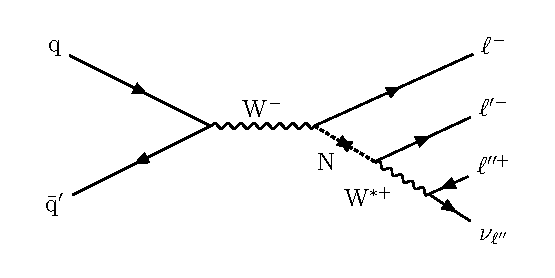
\includegraphics[width=0.24\textwidth]{Figures/c5/hnl_feyn.pdf}
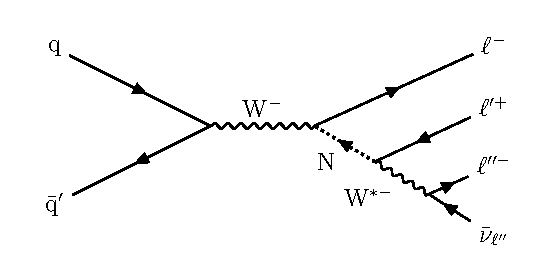
\includegraphics[width=0.24\textwidth]{Figures/c5/hnl_feyn_2.pdf}
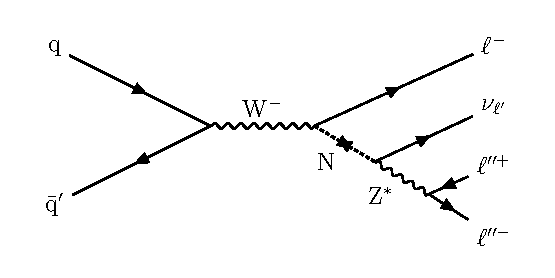
\includegraphics[width=0.24\textwidth]{Figures/c5/hnl_z_feyn.pdf}
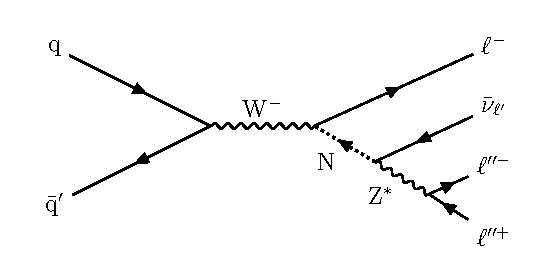
\includegraphics[width=0.24\textwidth]{Figures/c5/hnl_z_feyn_2.pdf}
\caption{Typical diagrams for the production of a HNL at the LHC 
($\hnl$) through its mixing with a SM neutrino, leading to a
final state with three charged leptons and a neutrino.}
\label{fig:c5hnldiagram}
\end{figure}

The final results of this analysis will be presented as a function of both the mass and the mixing parameter of the HNL's. 
The mixing parameter can depend on the flavor of the SM neutrino, so it has to be noted that the decays of the HNL 
might not be democratic across different lepton flavors.

The search for the HNL will be performed by binning the analysis in
variables that give discriminating power between signal and
background, and simultaneously fitting these search region to obtain
exclusion limits on the HNL signal as a function of its \mixpar and
mass. The latter analysis is almost fully blind to low mass signals as
it employs large thresholds on \met and relatively large lepton \pt
thresholds.



\section{Analysis setup}
\subsection{Data and simulation samples}
The current analysis uses a set of \Pp collision data corresponding to
an integrated luminosity of 35.9 \fbinv. Several primary datasets are used in this search due to the presence of all three
lepton flavors and a number of different control regions. (For precise
informations about the "primary dataset" see Chapter~\ref{Chapter2}.)

{\footnotesize
\begin{itemize}
\item DoubleEG
\item DoubleMuon
\item MuonEG
\item SingleMuon
\item SingleElectron
\end{itemize} }

A number of signal models, as described in the previous
Chapter~\ref{Chapter4}, were simulated with NLO precision. Signal
samples are generated with three leptons and a neutrino in the final
state, which includes N$\to\PW(\ell\nu)\ell$ and
N$\to\PZ(\ell\ell)\nu$ decay modes of the N. The \hnl masses of the
generated samples vary from 1\GeV to 1.2\TeV. 

The luminosity scenario has a 25~ns bunch crossing separation with an average of about 25 pileup interactions per bunch crossing.

\subsection{Signal compression and trigger strategy}\label{sec:compression}
A challenging aspect of the signal under consideration is that the \pt spectrum of the resulting leptons is in general compressed except for very high masses. The degree of this compression, and which leptons are affected, depends on the mass of the produced HNL. The \pt spectrum of the three hardest generator-level charged leptons is shown in figure~\ref{fig:genPt} for different HNL mass scenarios, ranging from 5 to 200 \GeV . 

\begin{figure}[h]
\subfloat[]{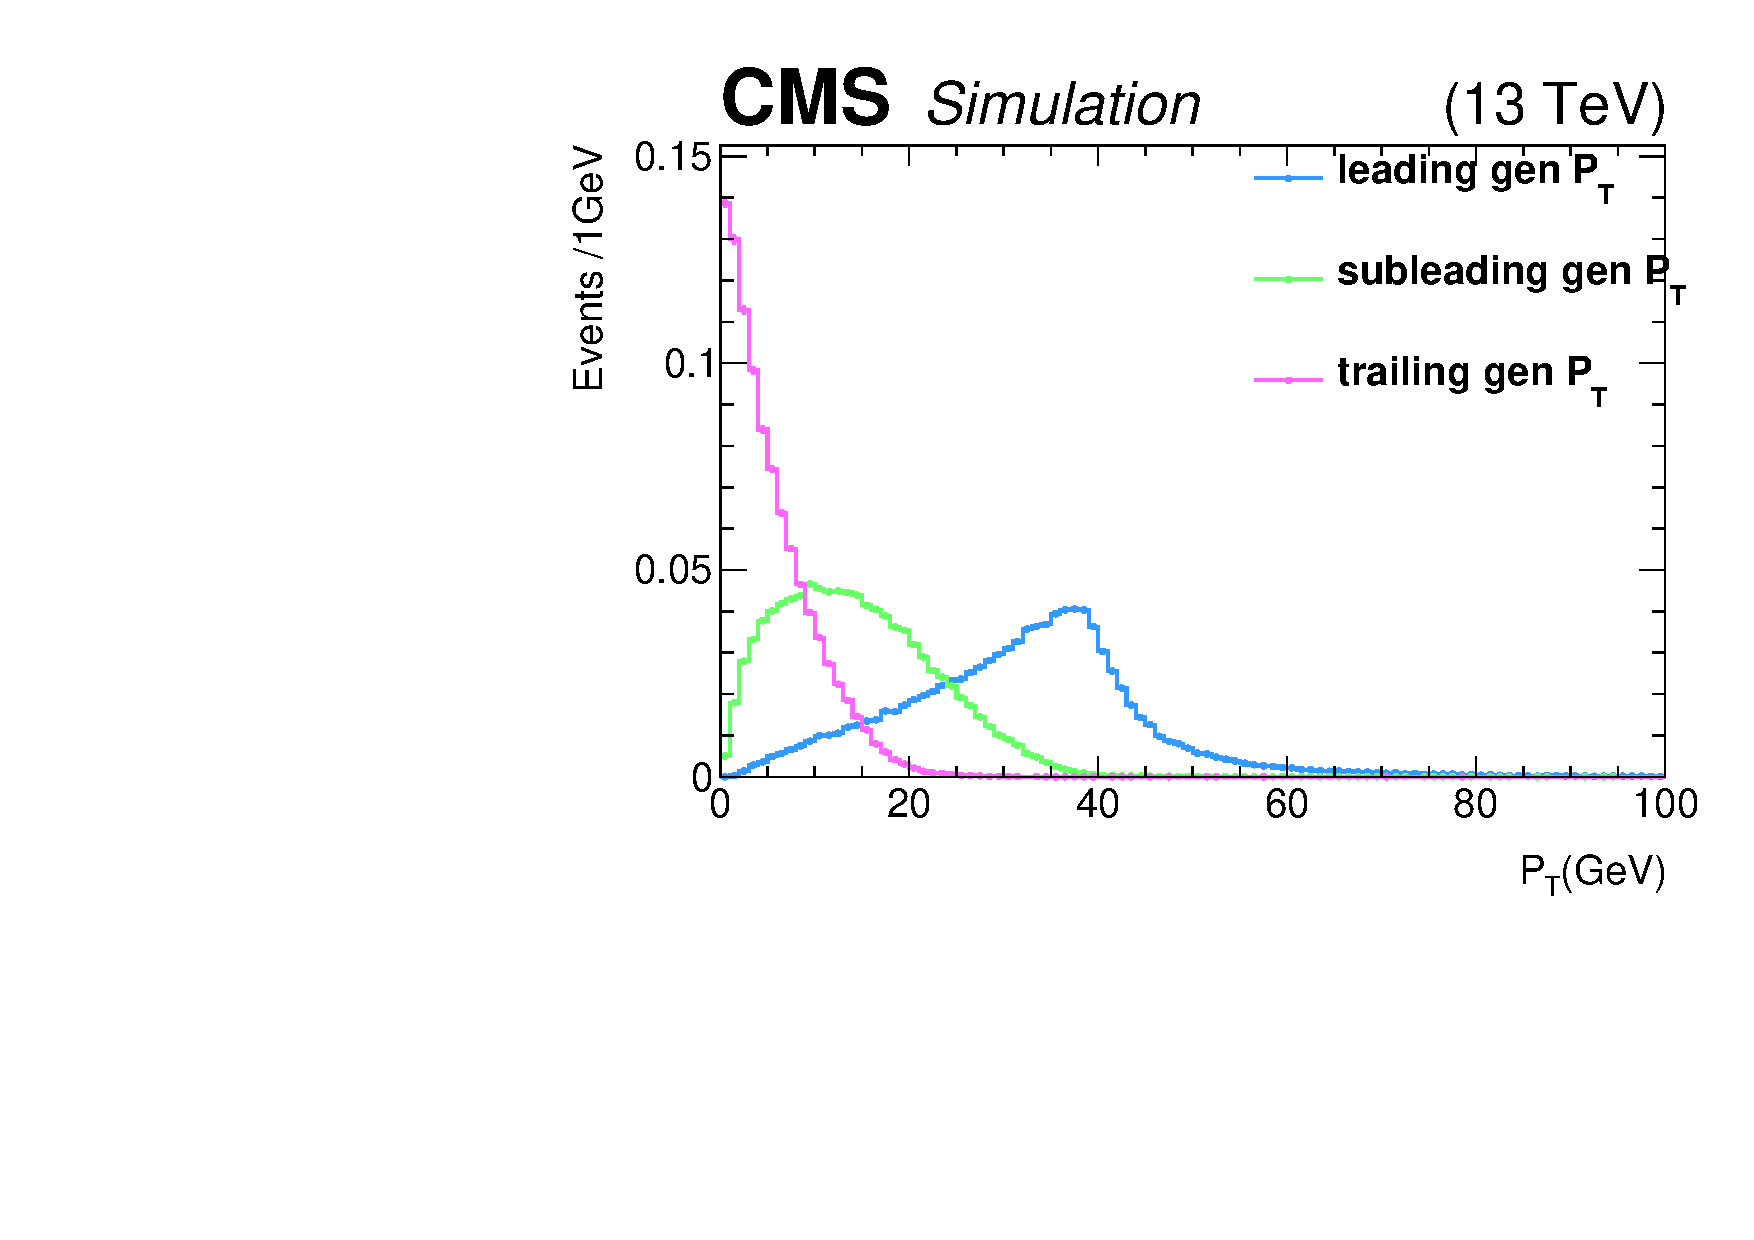
\includegraphics[width=.32\textwidth]{Figures/c5/genPt/genPtm5.pdf}}
\subfloat[]{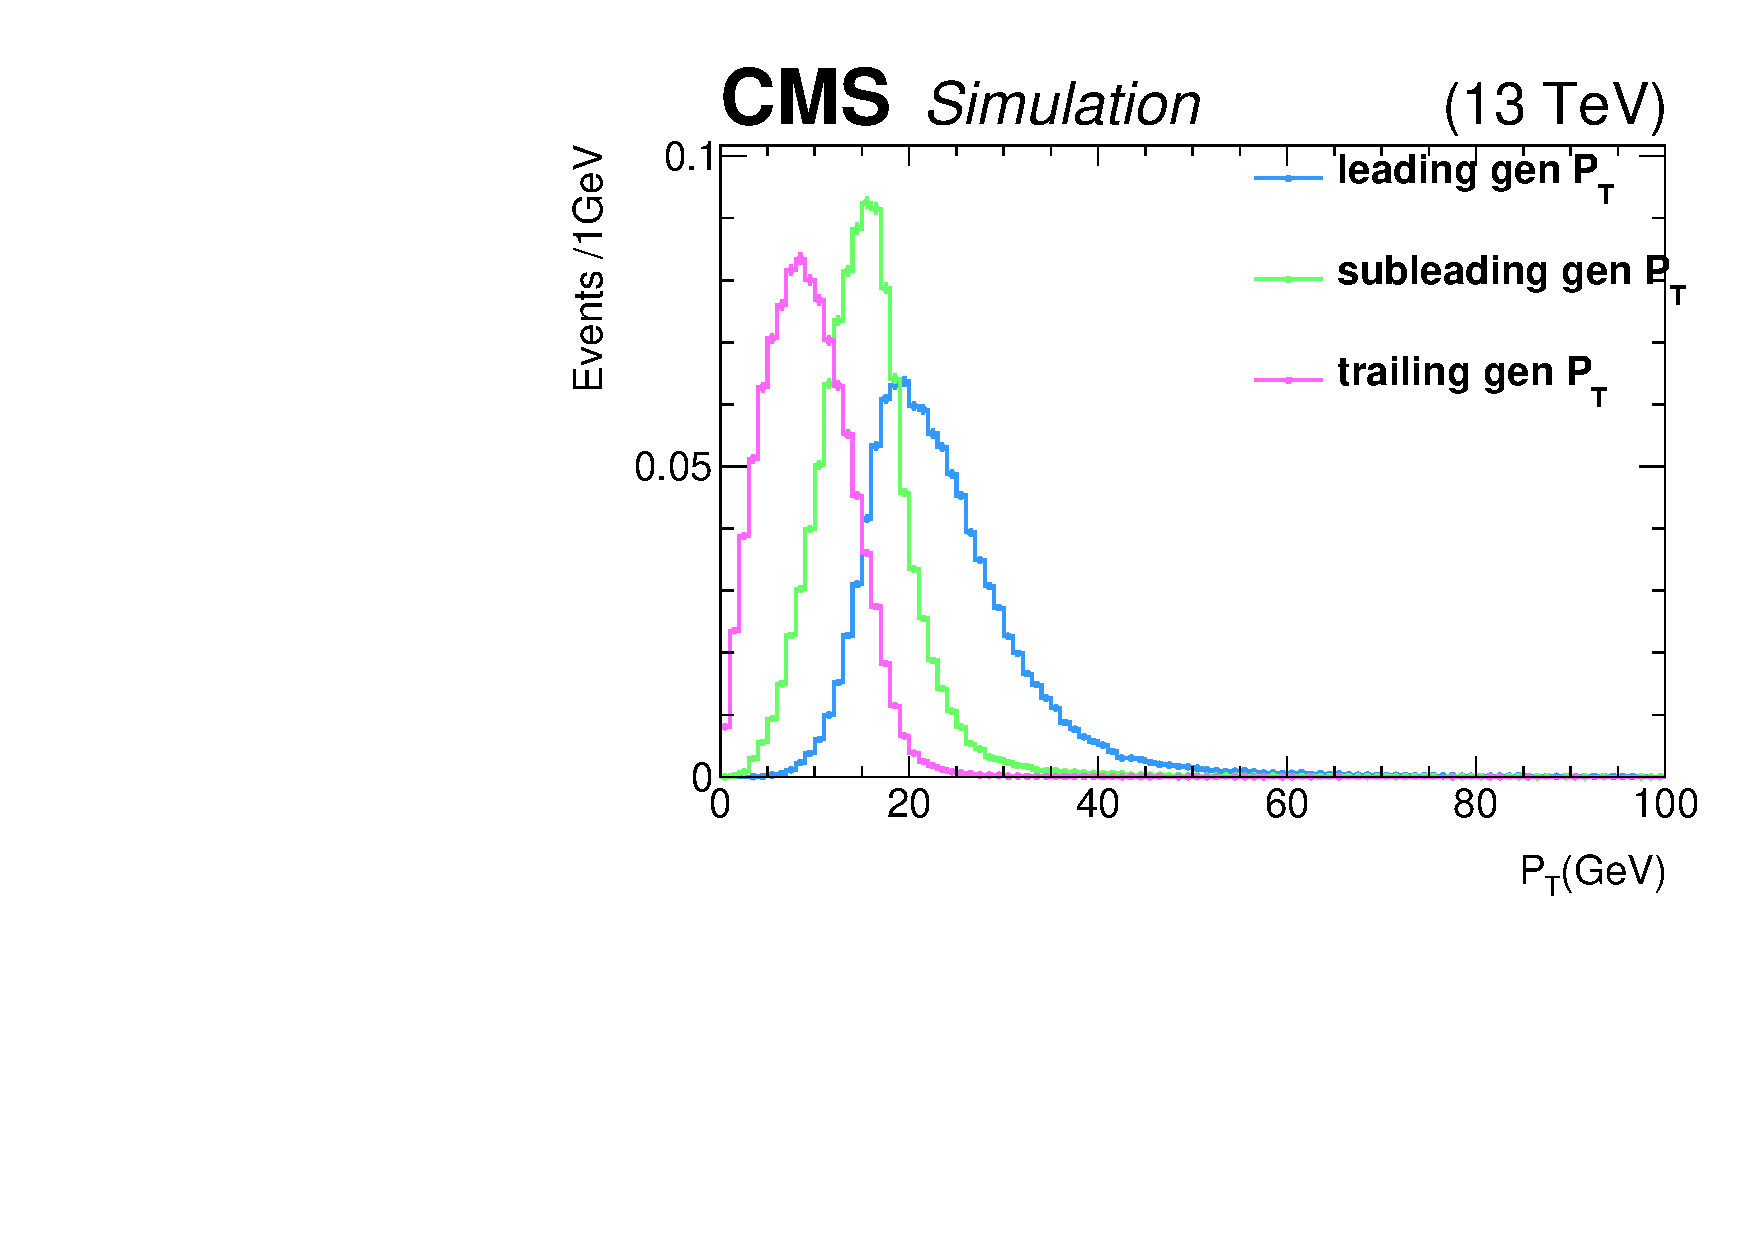
\includegraphics[width=.32\textwidth]{Figures/c5/genPt/genPtm60.pdf}}
\subfloat[]{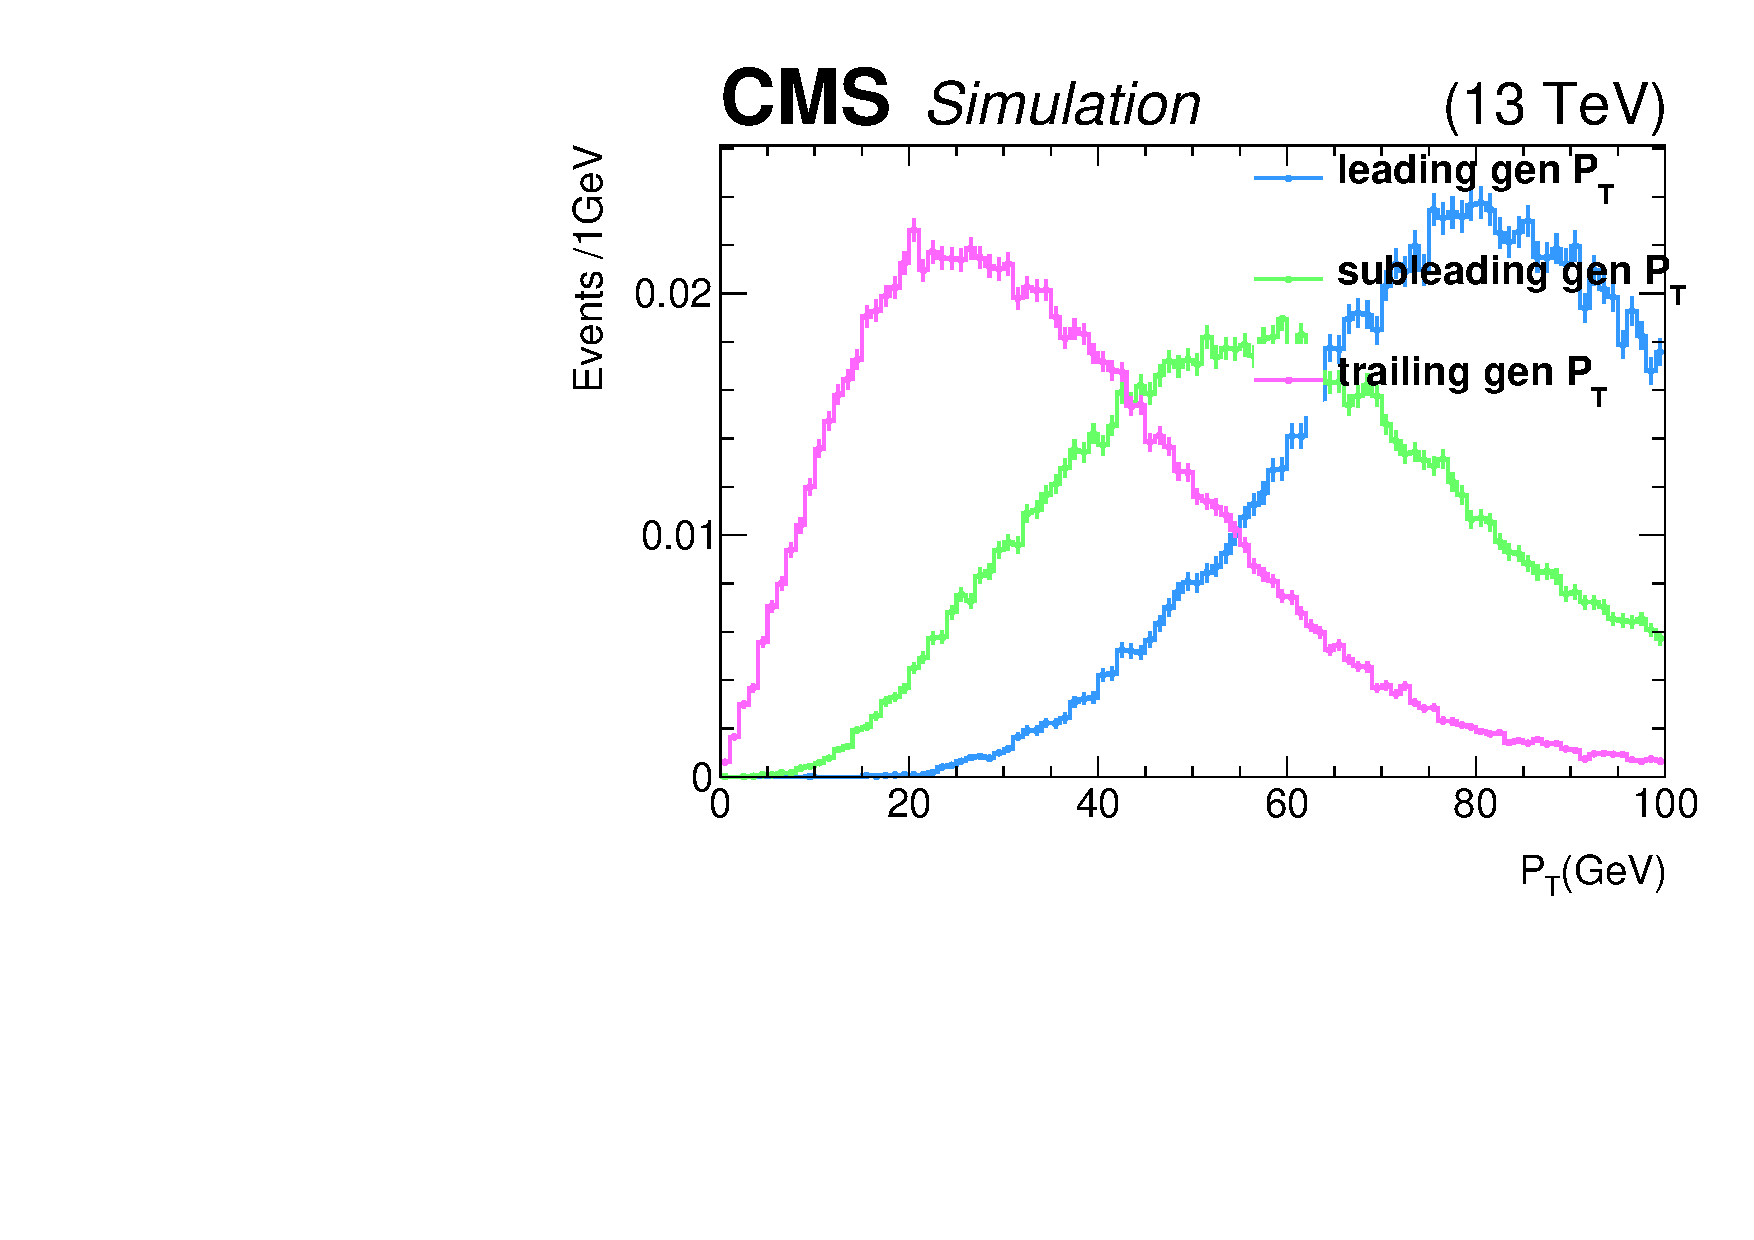
\includegraphics[width=.32\textwidth]{Figures/c5/genPt/genPtm200.pdf}}
\caption{\pt spectrum of the three hardest generator-level leptons in
  the signal simulation of several HNL masses. From top left to bottom
  right the HNL mass scenarios for which the spectrum is shown are 5
  \GeV (A), 60 \GeV (B), and 200 \GeV (C).}
\label{fig:genPt}
\end{figure}

It can be seen that for every mass scenario below the W-mass, one or
more leptons have a tendency to have very low \pt values. For low mass
samples both the trailing and sub-leading leptons are soft because of
the small mass of the decaying HNL. For masses close to the mass of
the W, very little phase space is left for the emission of the lepton
in the W's decay since all of the W's mass has to go into the
production of the HNL. For high masses on the other hand, the
compression is not as pronounced even though the trailing lepton can
still be seen to prefer relatively low momenta. The reason for the
compression of the trailing lepton is the fact that the W-boson has to
be highly off-shell to allow for the production of very heavy
HNL's. The cross section for off-shell W-boson production drops
rapidly with increasing mass, and as such the trailing lepton also
tends to have very little phase space available for its production in
very high mass scenarios.

We can clearly notice in Fig.~\ref{fig:genPt} different leptons \pt spectra according to the
$M_\hnl$ and its comparison wrt $M_\PW$. For this reason the analysis
strategy has been divided in two main phase spaces:
\begin{itemize}
\item \emph{low mass search:} soft leptons, $M_\hnl < M_\PW$;
\item \emph{high mass search:} hard leptons, $M_\hnl > M_\PW$;
\end{itemize}

\subsubsection{Trigger strategy}
Due to the low \pt spectra of the leptons in the HNL signals, designing a trigger strategy is a challenging task. 
For high HNL masses, the leading lepton \pt is generally above the efficiency turn on of the single-lepton triggers.
For low HNL masses, we need to add double- and triple-lepton triggers to obtain optimal signal efficiency.
The list of triggers used in this analysis are listed in table~\ref{table:HNL_trigger_thresholds}.


\begin{table}[h]
\centering
{\scriptsize
 \caption{Overview of the lepton \pt thresholds imposed in the analysis and the \pt regime in which each trigger path provides sensitivity.}
  \label{table:HNL_trigger_thresholds}
  \begin{tabular}{c|c|ccc|l}
   \hline
    search region                  & lepton flavors                    & \multicolumn{3}{c|}{selected \pt range (\GeV)} & sensitive trigger paths \\
                                   & $\ell^{\text{leading}} \; \ell^{\text{subleading}} \; \ell^{\text{trailing}}$ & $\pt^\text{leading}$ & $\pt^\text{subleading}$ & $\pt^\text{trailing}$ & \\
    \hline
    \multirow{12}{*}{low mass}     & $ee\mu$                           & 30--55 & $>15$    & $>5$     & $1e$ \\
                                   &                                   & 15--30 & $>15$    & $>8$     & $2e1\mu$ \\
                                   &                                   & 23--30 & 10--15    & $>8$     & $1e1\mu$ \\
                                   &                                   & 25--30 & $>15$    & 5--8      & $2e$ \\
                                   & $e\mu e$, $\mu ee$                 & 30--55 & $>15$    & $>10$    & $1e$ or $1\mu$ \\
                                   &                                   & 15--30 & $>15$    & $>15$    & $2e1\mu$ \\
                                   &                                   & 23--30 & $>10$    & 10--15    & $1e1\mu$ \\
                                   & $\mu\mu e$                        & 30--55 & $>15$    & $>10$    & $1\mu$ \\
                                   &                                   & 15--30 & $>10$    & $>10$    & $1e2\mu$ \\
                                   & $\mu e \mu$, $e\mu\mu$            & 30--55 & $>10$    & $>10$    & $1e$ or $1\mu$ \\
                                   &                                   & 15--30 & $>10$    & $>9$     & $1e2\mu$ \\
                                   &                                   & 23--30 & $>10$    & 5--9      & $1e1\mu$ \\
    \hline
    high mass                      & all flavors
                                                                       & $> 55$    & $>15$    & $>10$  & all paths \\
 \hline
  \end{tabular}
}
\end{table}

The overall approach to selecting the offline thresholds in the analysis is the following:

\begin{itemize}
\item calculate trigger data/MC scale factors (SF) for each lepton-specific trigger and determine values where these SF = const. Typical SF value: 98\% for a muon-specific and 99\% for an electron-specific. 
\item determine total efficiency of trigger combinations (~\ref{table:HNL_trigger_thresholds}) in MC simulation, and choose \pt thresholds leading to the high overall efficiency and being not lower than the values determined in the first step;
\item check the overall data/MC SF in a orthogonal dataset which was
  selected without using lepton trigger to avoid unavoidable biases;
\item determine systematics from the SF values obtained in the first step and validate its choice in the previous step: 
\begin{itemize}
\item use 5\% systematics for events with leading lepton $\pt < 30$\GeV (max. SF value for $\Pe\Pe\mu$ and $\Pe\mu\mu$ case),
\item and 2\% for events with leading lepton $\pt > 30$\GeV (max. SF value of a muon leg).
\end{itemize}
\item require trigger information in MC samples when deriving the yields, but not apply any additional correction.
\end{itemize}

We use the tag-and-probe method to measure the lepton-specific efficiencies. The efficiency is 
defined as the ratio of selected events where the probe matches the lepton-specific in question ($\Delta R<0.4$) over 
the total number of selected events. Events entering the denominator in data are taken from the 
SingleElectron (SingleMuon) dataset and must fire an unprescaled
single lepton trigger with \pt threshold > 27\GeV (> 24\GeV).

Requiring the tag and the probe to both pass the offline lepton selection reduces the contamination 
from fakes at sub-percent level. We therefore do not perform any background subtraction using a fit to 
the \PZ peak. This choice presents the advantage that the measurement in channels purely dominated by the 
Drell-Yan process ($\Pe\Pe$ and $\mu\mu$) can be compared to a channel where the contribution from \ttbar 
becomes dominant at high lepton $\pt$ ($\Pe\mu$).

In order to estimate the uncertainty on the trigger efficiency for the OR combination of single, double and trilepton triggers,
we select trilepton events according to the baseline selection criteria described in Section~\ref{sec:object}.
The trigger efficiency is then measured as a function of the trailing
lepton \pt in both the unbiased \verb!MET! dataset, a high-statistics $\PW\PZ$ MC sample and a HNL samples. 
The applied baseline selection criteria
ensures we are on the efficiency plateau, see Fig.~\ref{fig:3l1l1lEff}, and reasonable data/MC agreement is observed 
as statistical uncertainties of the samples allow to judge.

The overall $1\ell+2\ell+3\ell$ trigger efficiency as measured in WZ MC samples 
after selecting 3 leptons with relevant flavor combination which pass
the offline analysis ID is typically close to 100\%, and is not lower
than 92\%, for events with leading lepton has $\pt > 30$\GeV. For
events when the leading lepton has $\pt < 30$\GeV, the efficiency
falls down reaching the value of 70\% in the worst case scenario.
Thus we assign a 5\% uncertainty
on the trigger efficiency for a leading lepton $\pt < 30$\GeV $\;$which corresponds to data/MC SF value 
for the total of three lepton-specific of trilepton triggers.
As the single-lepton trigger reaches its plateau for $\pt > 30$\GeV,
events with leading lepton $\pt > 30$\GeV$\;$are assigned a 2\%
uncertainty which corresponds to the the largest of the SF of muon and electron specifics. 


\begin{figure}[h]
  \centering
  \subfloat[{\tiny$3\Pe$, $\pt^\text{lead} > 55\GeV$}]{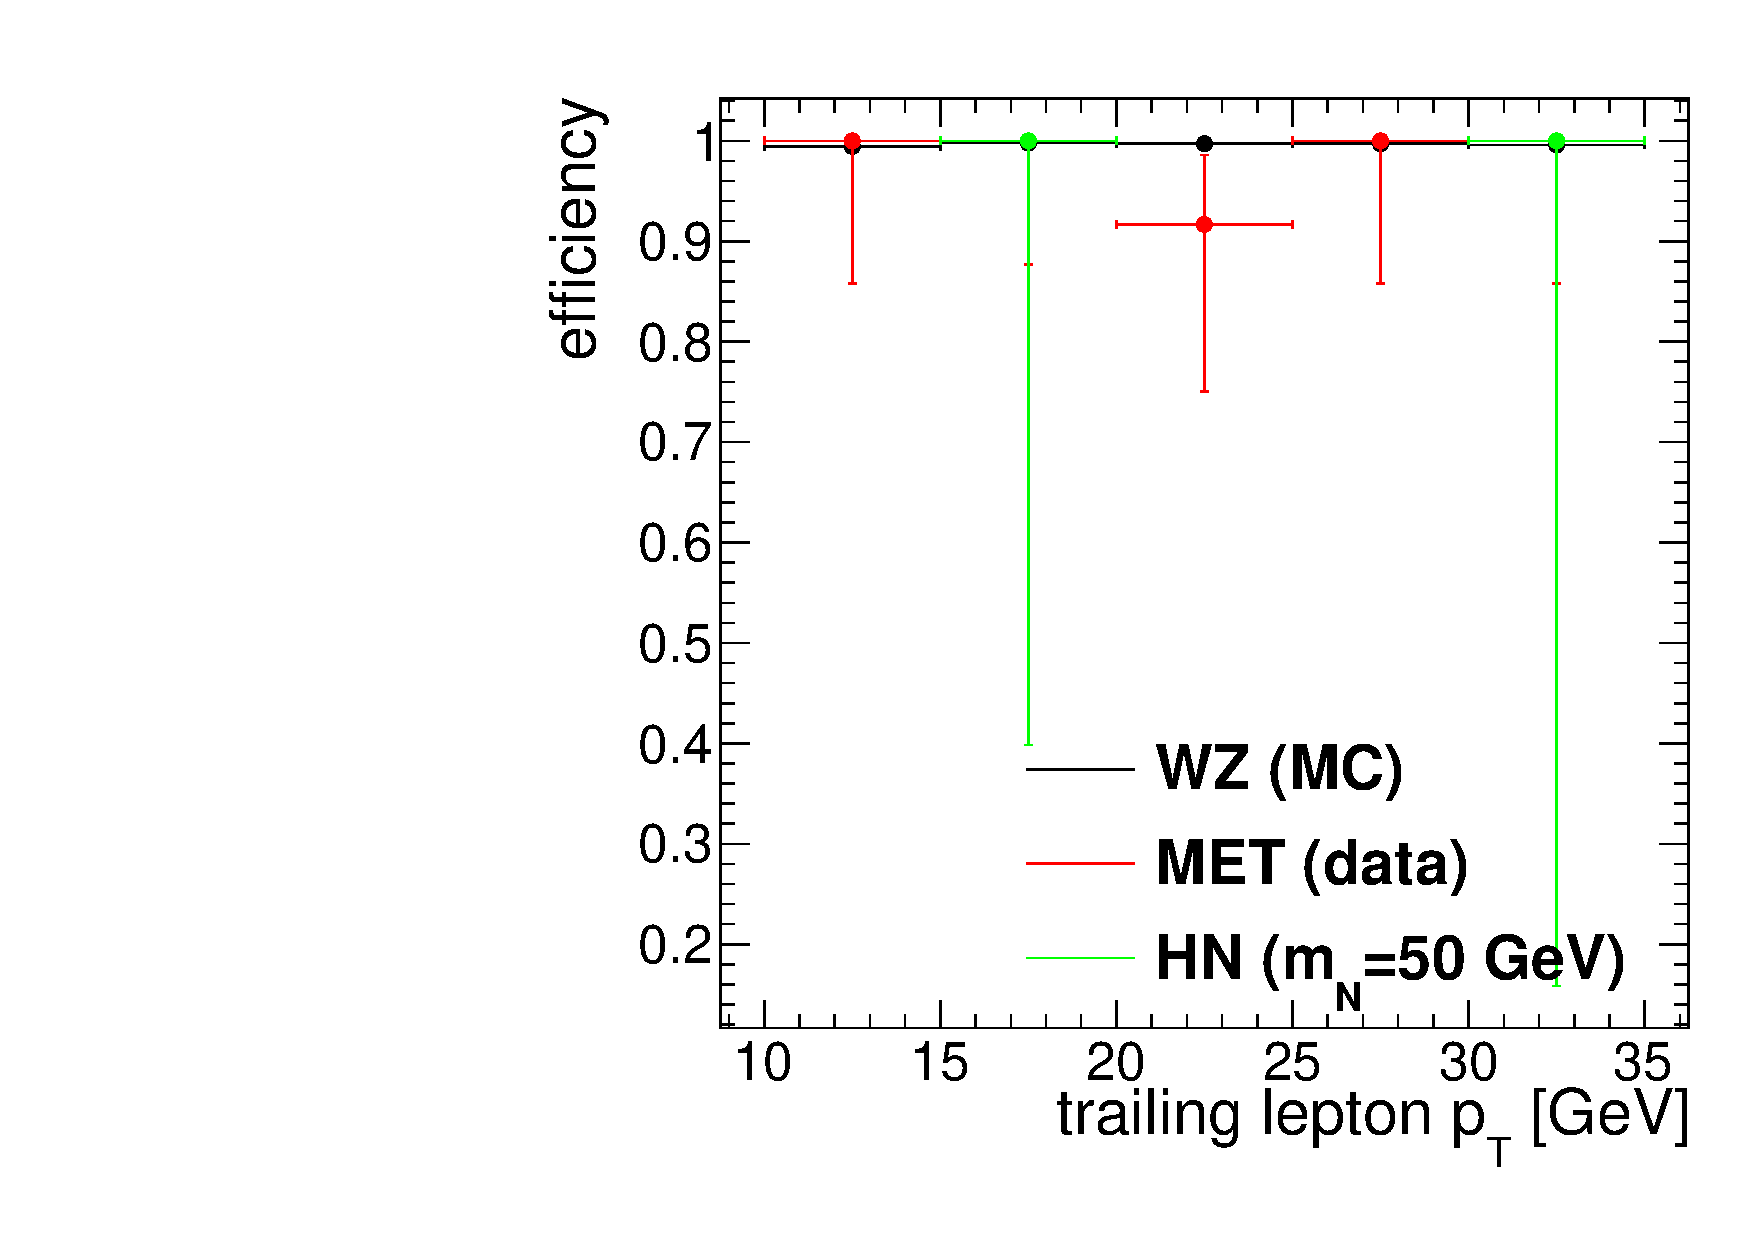
\includegraphics[width=0.32\textwidth]{Figures/c5/trigger/vsTrailingPt/eee_pt55to1000.pdf}}
  \subfloat[{\tiny$3\mu$, $\pt^\text{lead} > 55\GeV$}]{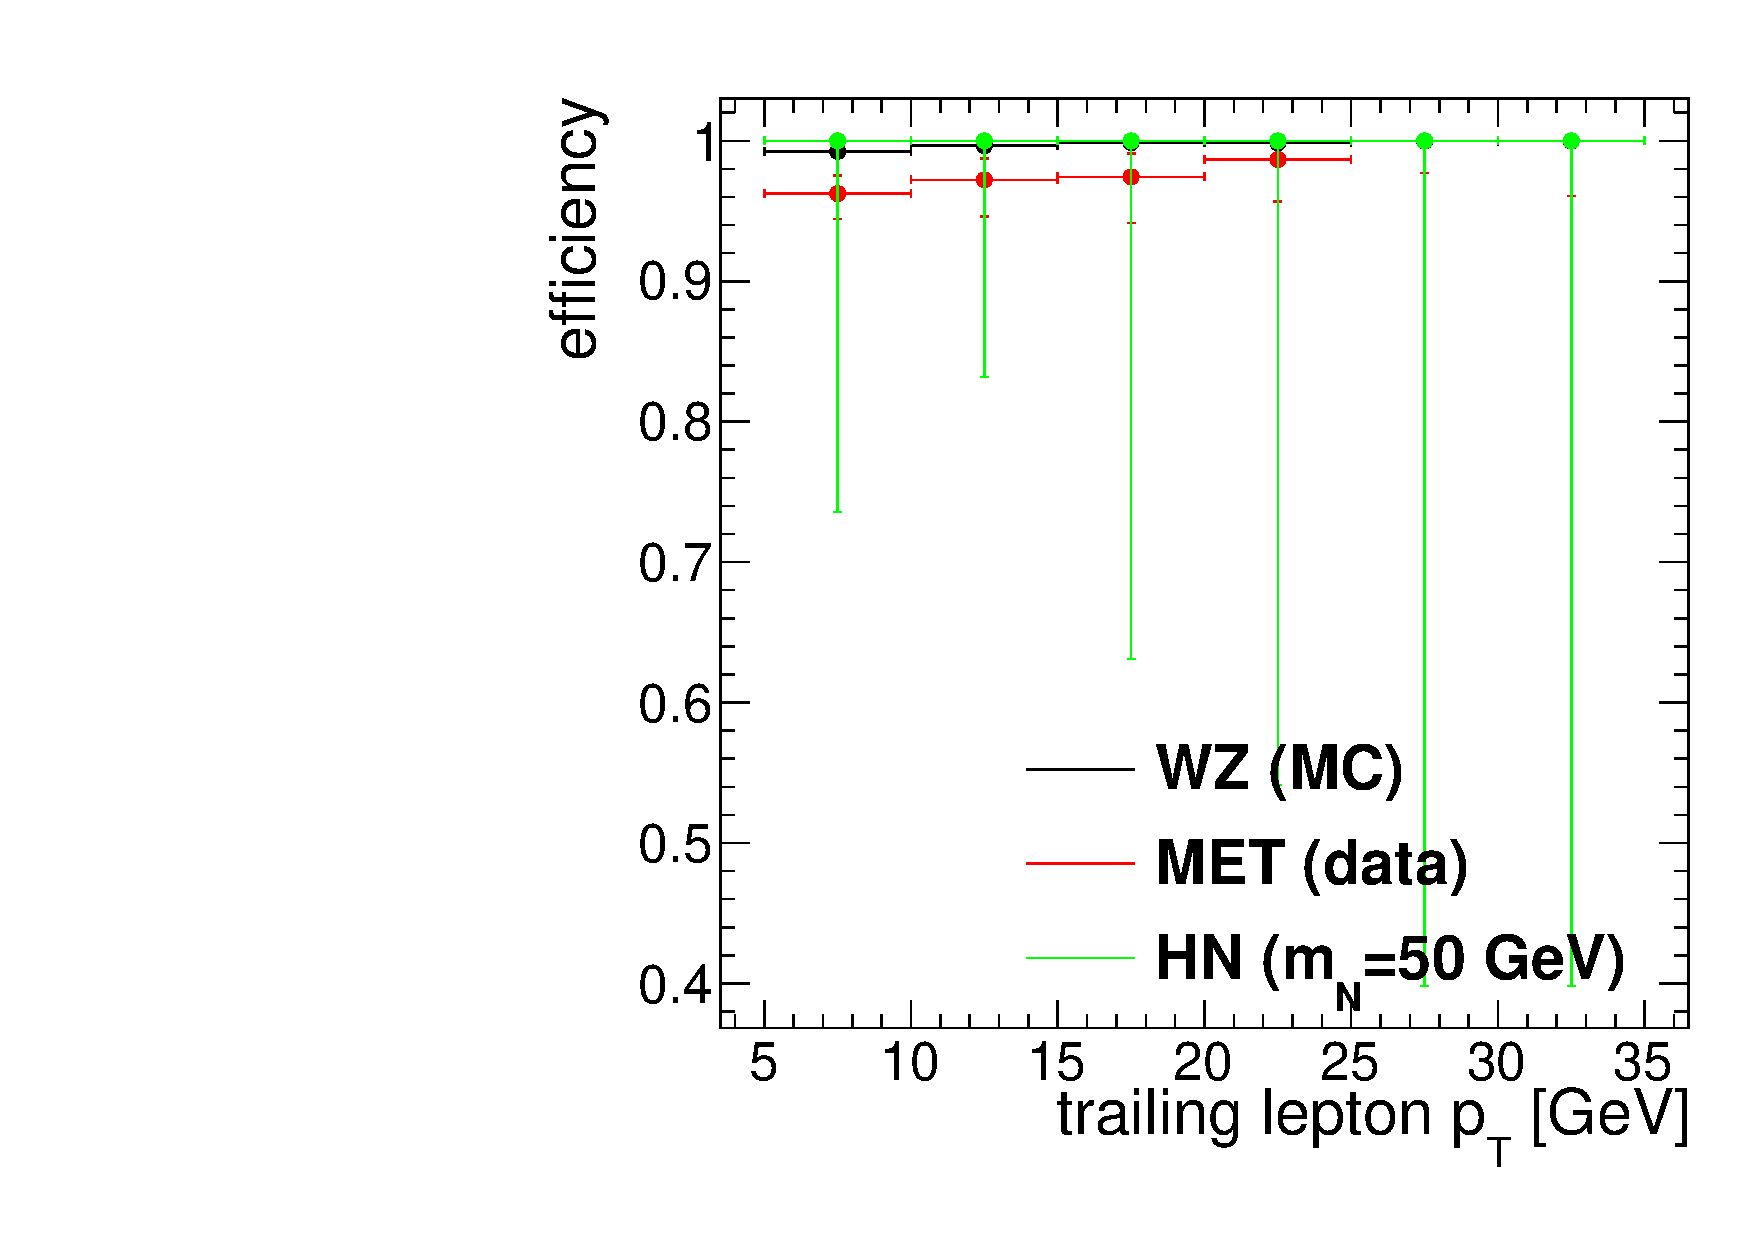
\includegraphics[width=0.32\textwidth]{Figures/c5/trigger/vsTrailingPt/mumumu_pt55to1000.pdf}} 
  \subfloat[{\tiny$2\Pe1\mu$, $\pt^\text{lead} [15,30] $}]{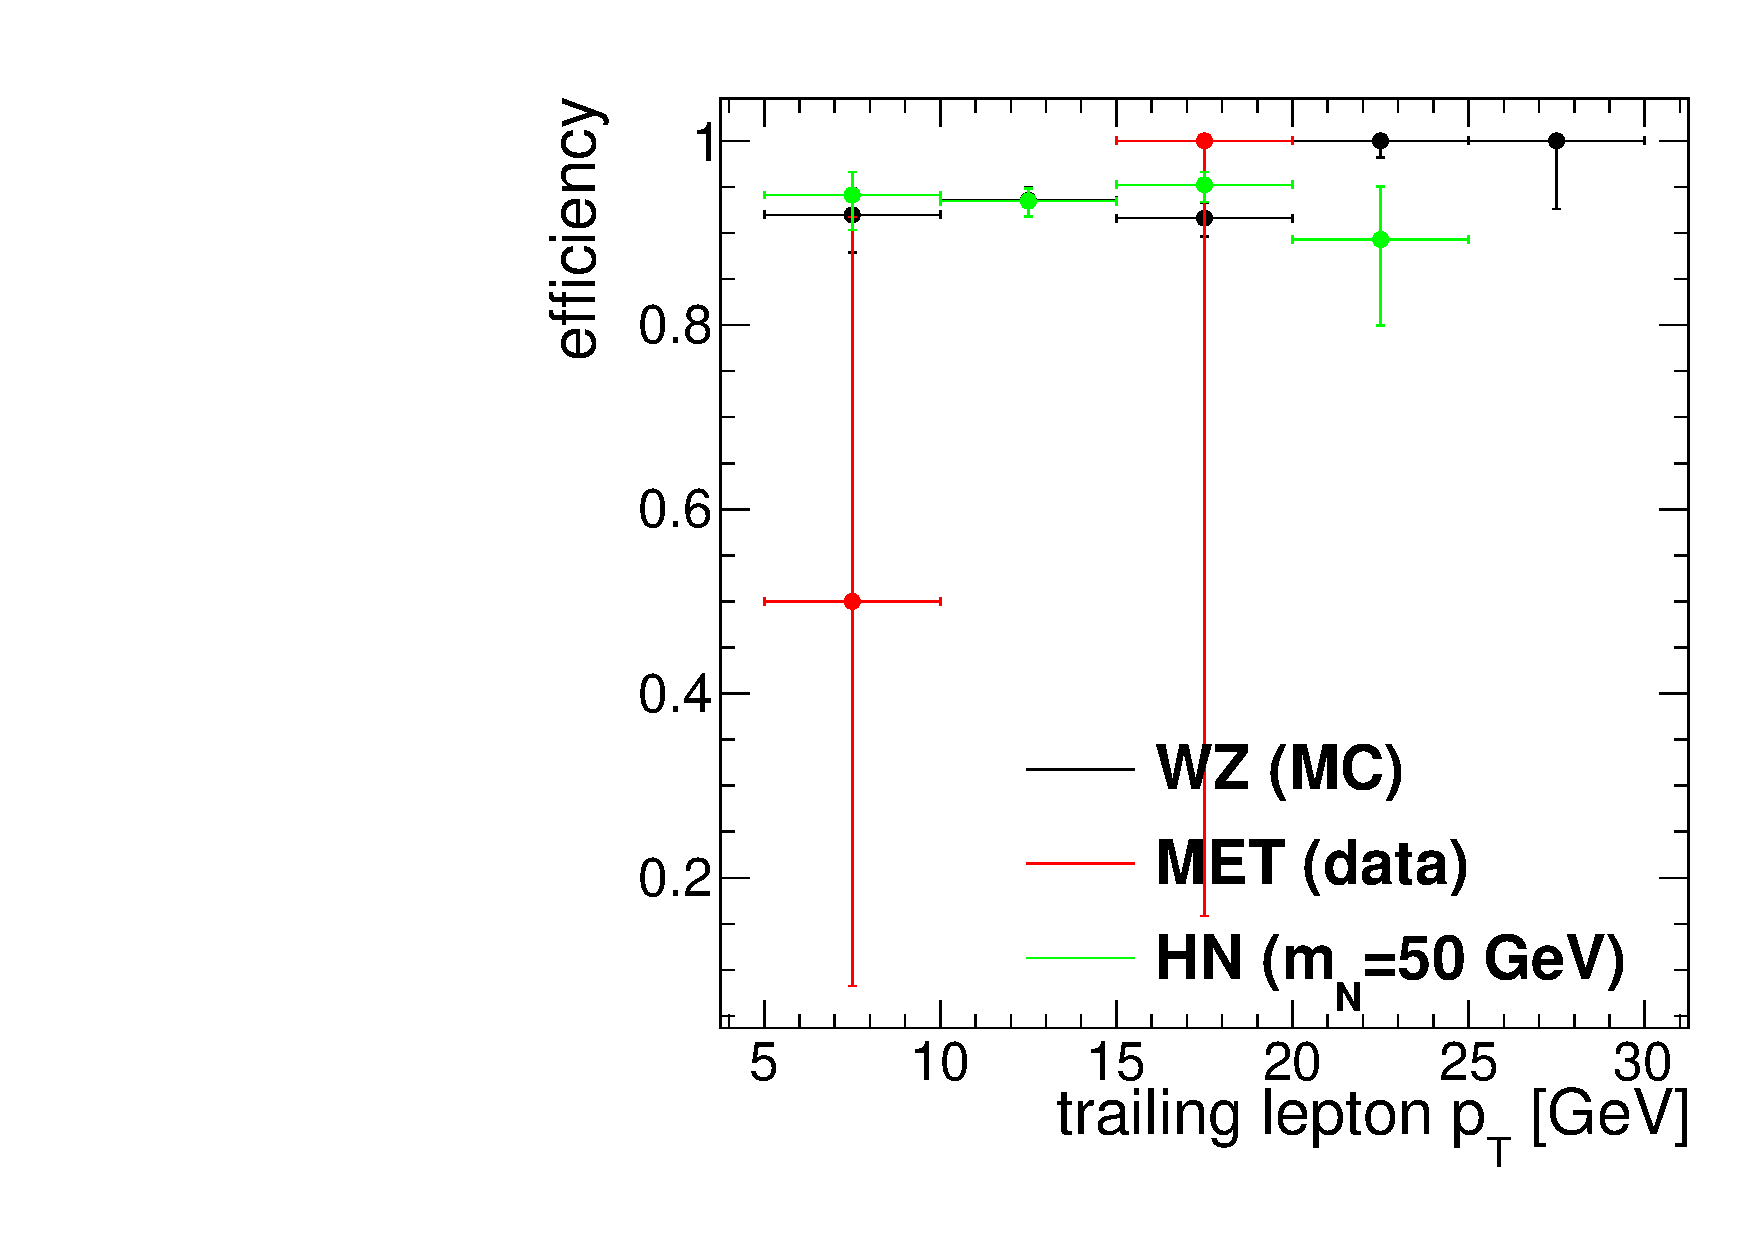
\includegraphics[width=0.32\textwidth]{Figures/c5/trigger/vsTrailingPt/eemu_pt0to30.pdf}}\\
  \subfloat[{\tiny$2\Pe1\mu$, $\pt^\text{lead} [30,55] $}]{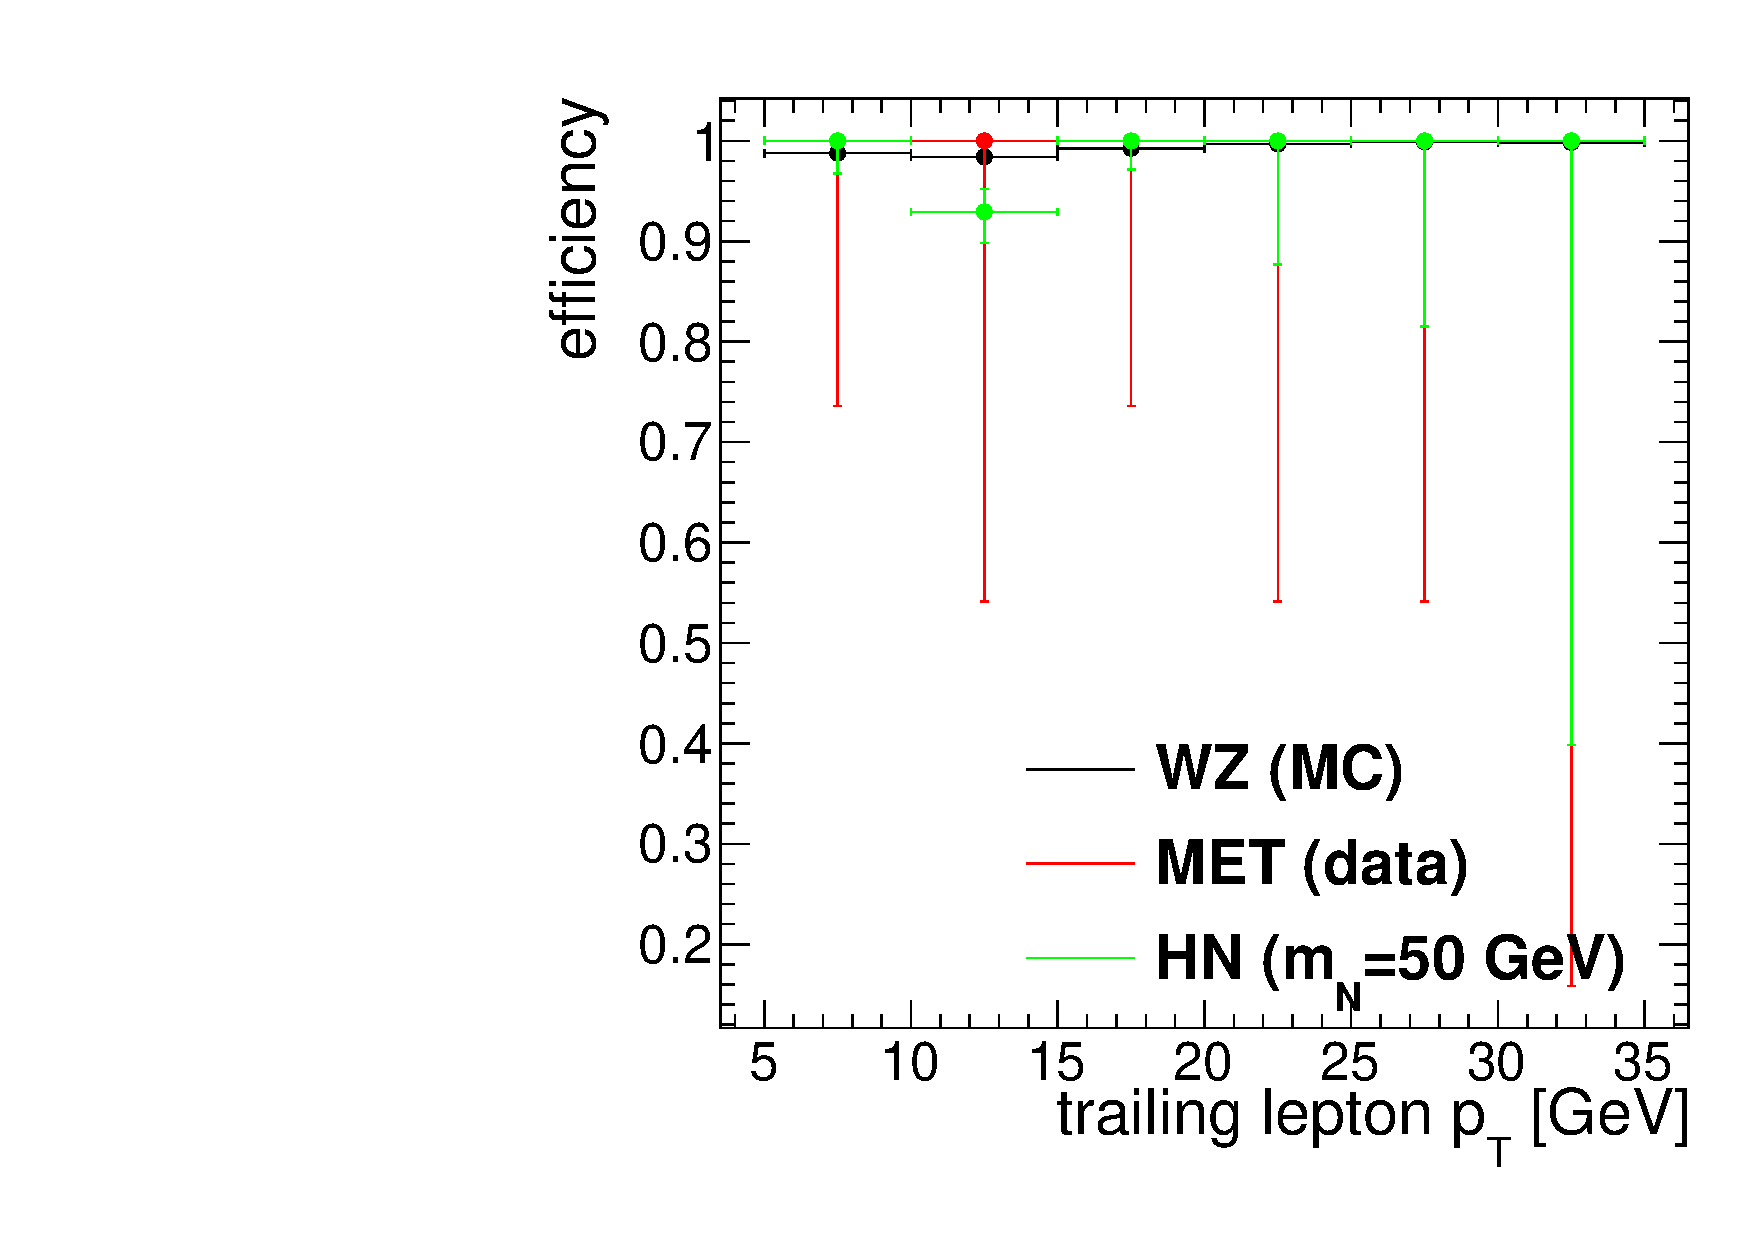
\includegraphics[width=0.32\textwidth]{Figures/c5/trigger/vsTrailingPt/eemu_pt30to55.pdf}} 
  \subfloat[{\tiny$1\Pe2\mu$, $\pt^\text{lead} [15,30] $}]{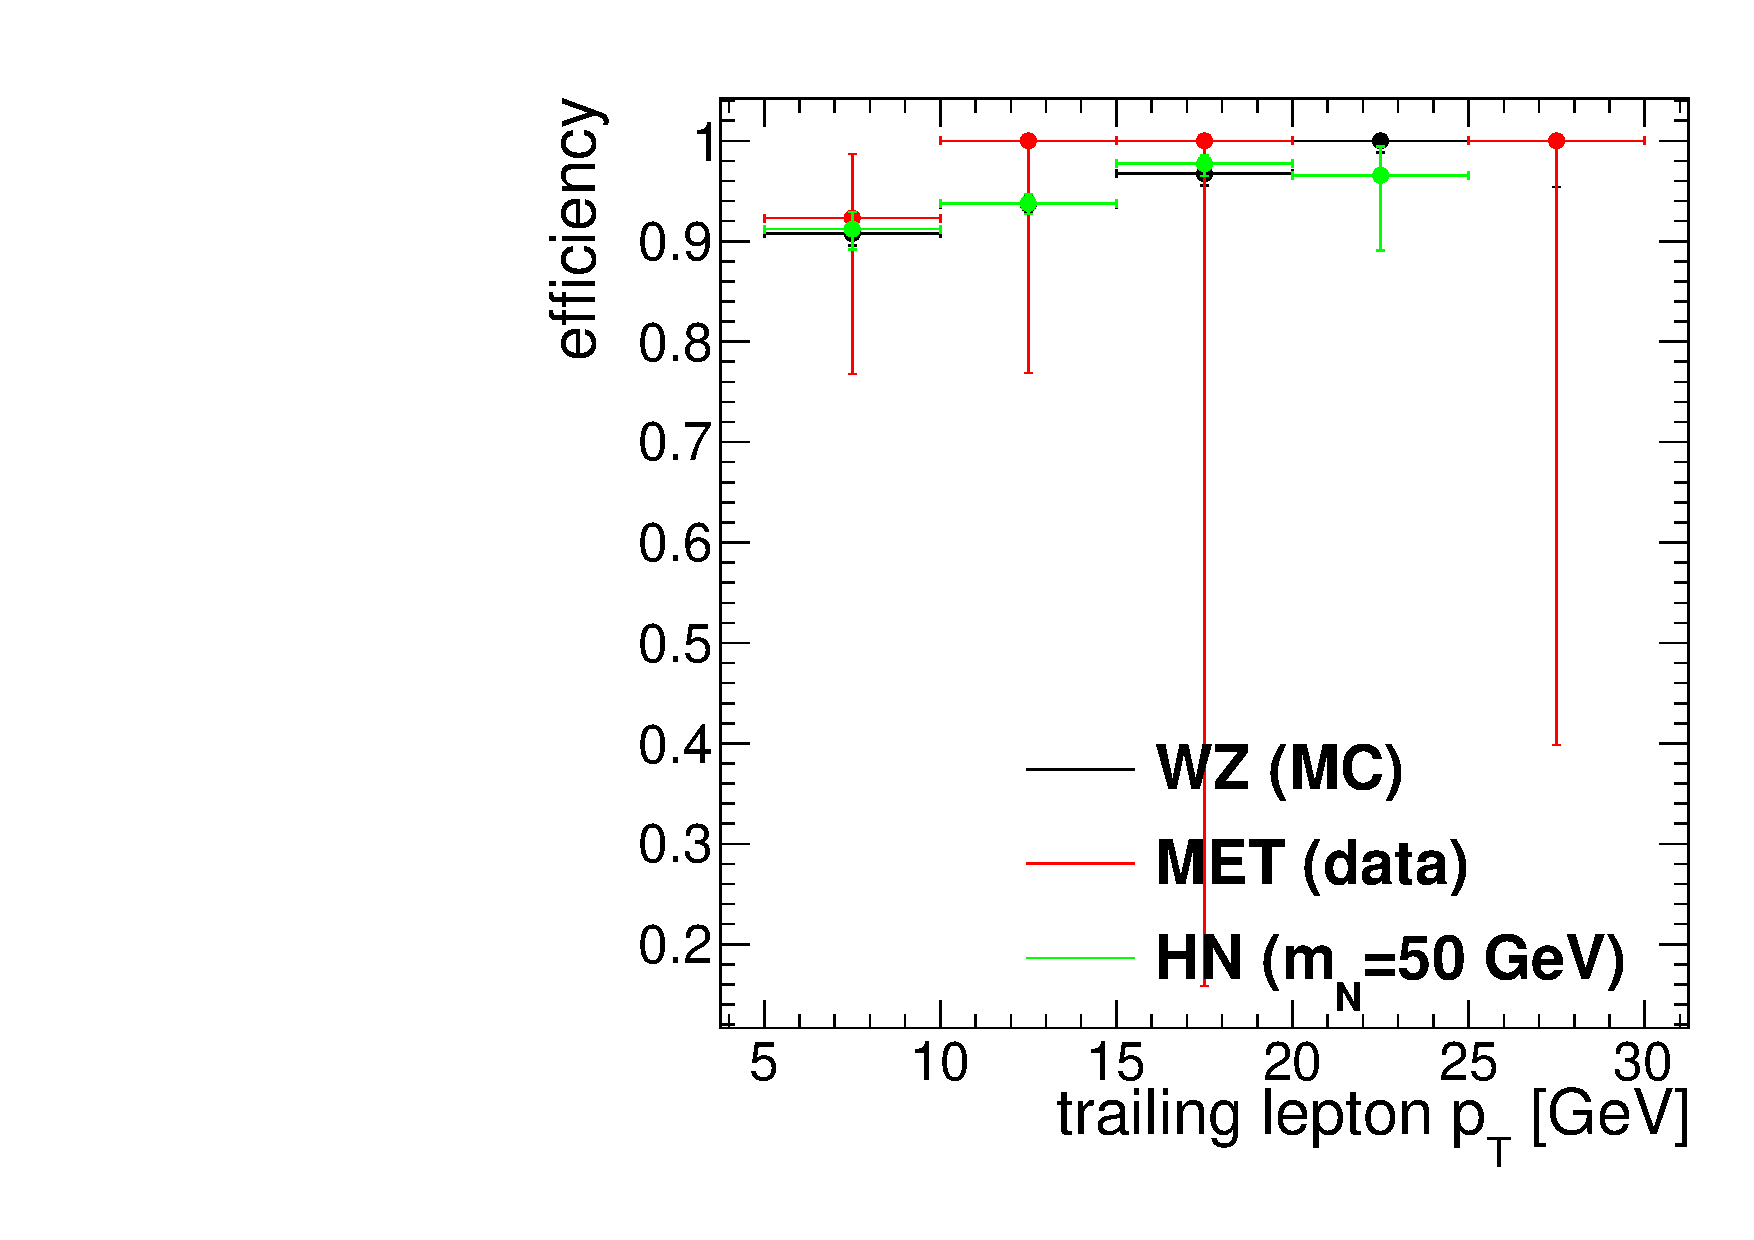
\includegraphics[width=0.32\textwidth]{Figures/c5/trigger/vsTrailingPt/emumu_pt0to30.pdf}}
  \subfloat[{\tiny$1\Pe2\mu$, $\pt^\text{lead} [30,55] $}]{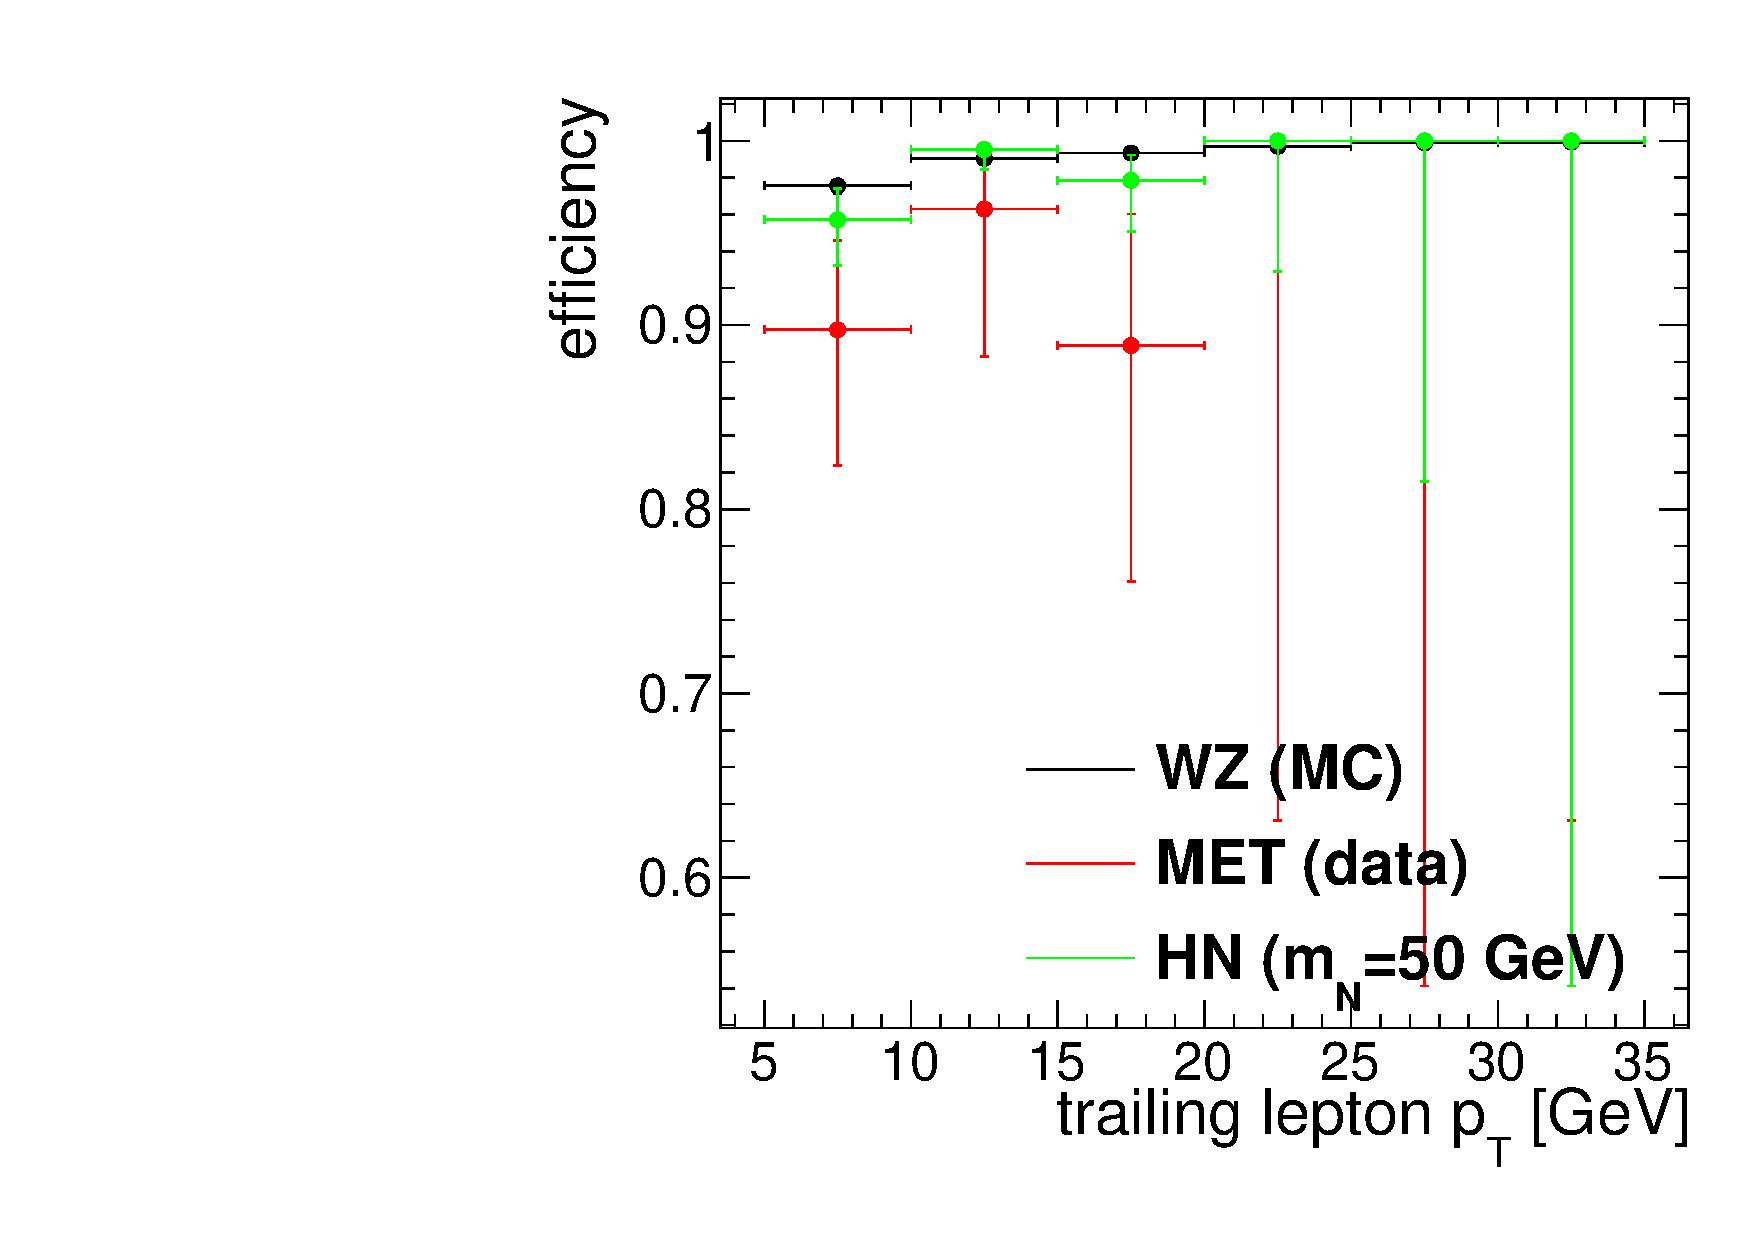
\includegraphics[width=0.32\textwidth]{Figures/c5/trigger/vsTrailingPt/emumu_pt30to55.pdf}} \\
  \caption{Efficiencies for the OR combination of single, double and trilepton triggers, in trilepton events as a function
  of the trailing lepton \pt.}
  \label{fig:3l1l1lEff}
\end{figure}

\subsection{Object selection}\label{sec:object}
For the rigorous explanation of the single object reconstruction in
CMS see Chapter~\ref{Chapter2}, section~\ref{sec:reconstruction}.

\subsubsection{Leptons}
The base objects of this analysis are electrons and muons. Both electrons and muons have three selection working points, called "loose", "fakeable object" (FO) and "tight". The loose working point is used when cleaning electrons from overlap with muons, to be specific, electrons are not considered for selection if they fall within a cone of $\Delta \mathrm{R} = 0.05$ around a loose muon. The FO working point is slightly tighter than the loose one, and is extensively used for the estimation of the background due to non-prompt and fake leptons as described further in this text. The crucial property of the FO working point is that the probability for a non-prompt lepton passing the FO working point to also pass the tight working point is almost independent of the flavor of the jet or hadron from which the fake lepton originates. This property will prove essential for the non-prompt lepton background estimation as further specified. The full definitions of every selection working point, for respectively muons and electrons are shown in tables ~\ref{tab:muonIDs} and \ref{tab:eleIDs}.

An isolation variable (\Irel) is computed as the ratio of the scalar 
\pt sum of charged hadrons originating from the PV, neutral hadrons, and photons within a cone of 
$\Delta R<0.3$ around the lepton candidate direction at the vertex, 
to the transverse momentum $\pt^\ell$ of the lepton candidate. 
"Loose" and "fakeable object" leptons are required to have $\Irel < 0.6$. 
"Tight" leptons must satisfy $\Irel < 0.1$.

\begin{table}[h!]
\centering
{\scriptsize
\caption{
Requirements to pass each definition of the muon selection.}
\label{tab:muonIDs}
\begin{tabular}{c|c|c|c}
\hline
\bf{Cut} & \bf{Loose} & \bf{Fakeable Object} & \bf{Tight} \\
\hline
$|\eta| < 2.4$ & \checkmark & \checkmark & \checkmark \\
$\pt$ & $>5$ & $>5$ & $>5$\\
$|d_{xy}| < 0.05$ (cm) & \checkmark & \checkmark & \checkmark \\
$|d_z| < 0.1$ (cm) & \checkmark & \checkmark & \checkmark \\
$\text{SIP}_{3D} < 4$ & -- & \checkmark & \checkmark \\
$\Irel$ & $<0.6$ & $<0.6$ & $<0.1$ \\
is PF Muon & \checkmark & \checkmark & \checkmark \\
is Global or Tracker Muon & \checkmark & \checkmark & \checkmark \\
is POG Medium Muon & -- & \checkmark & \checkmark \\
\hline
\end{tabular}
}
\end{table}


\begin{table}[h!]
\centering
{\scriptsize
\caption{
Requirements for an electron to pass each of the defined working points. Two POG MVA thresholds are given for respectively 15, and 25\GeV . Electrons above 25\GeV$\:$or below 15\GeV$\:$are required to pass the corresponding working point, while a linearly decreasing cut between the two working points is applied to electrons with a \pt inbetween these values. For every MVA working point three values are given corresponding to electrons with $0 < |\eta| < 0.8$, $0.8 < |\eta| < 1.479$, and $1.479 < |\eta| < 2.5$.
}
\label{tab:eleIDs}
\resizebox{1.0\linewidth}{!}{
\begin{tabular}{c|c|c|c}
\hline
\bf{Cut} & \bf{Loose} & \bf{Fakeable Object} & \bf{Tight} \\
\hline
$|\eta| < 2.5$ & \checkmark & \checkmark & \checkmark \\
$\pt$ & $>10$ & $>10$ & $>10$ \\
$|d_{xy}| < 0.05$ (cm) & \checkmark & \checkmark & \checkmark \\
$|d_z| < 0.1$ (cm) & \checkmark & \checkmark & \checkmark \\
$\text{SIP}_{3D} < 4$ & -- & \checkmark & \checkmark \\
\Irel & $<0.6$ & $<0.6$ & $<0.1$ \\
POG MVA ID (\pt $<$ 15 $\mathrm{GeV}$)& -- & $> (-0.02, -0.52, -0.52)$ & $> (0.77, 0.56, 0.48)$\\
POG MVA ID (\pt $>$ 25 $\mathrm{GeV}$)& -- & $> (-0.02, -0.52, -0.52)$ & $> (0.52, 0.11, -0.01)$\\
$\sigma_{i\eta i\eta} <(0.011,0.011,0.030)$ & -- & \checkmark & \checkmark \\
H/E $< (0.10,0.10,0.07)$ &  -- &  \checkmark & \checkmark \\
$\Delta\eta_{\textrm in} < (0.01, 0.01, 0.008)$ & -- & \checkmark & \checkmark \\
$\Delta\phi_{\textrm in} < (0.04, 0.04, 0.07)$ & -- & \checkmark & \checkmark \\
$-0.05 < 1/E-1/p < (0.010,0.010,0.005)$ & -- & \checkmark & \checkmark \\
conversion rejection & \checkmark & \checkmark & \checkmark \\
Number of missing hits & $<2$ & $== 0$ & $== 0$ \\
\hline
\end{tabular}}
}
\end{table}

A notable difference between the muon and electron selection criteria
are the \pt thresholds that are being used. Considering the earlier
discussion on the compressed \pt spectra of the target signal, it is
clear that we want to apply \pt thresholds as low as feasible in order
to gain the maximum signal efficiency. So ideally we would want low
\pt thresholds on both muons and electrons, but the triggers are a
limiting factor in how low we can realistically go. The higher
electron trigger thresholds make going lower than 10\GeV $\:$in electron \pt unfeasible, even though our trigger strategy is
optimized for maximum efficiency and thresholds as low as possible, as
described in the previous section. The relatively high \pt thresholds forced upon us by the available
triggers leave us with relatively low signal efficiencies, as the
often very soft trailing, and subleading signal leptons do not manage
to pass the thresholds of the baseline object selection.
 Aside from this, harsher \pt thresholds of 15 and 10\GeV $\:$are applied
 to the leading and subleading leptons in order to pass the employed
 triggers.

\subsubsection{Jet selection and $p_{T}^{miss}$}
Particle-flow candidates are clustered into jets using the anti-$k_t$ algorithm~\cite{Cacciari_2008} with a distance parameter of 0.4, 
as implemented in the \FASTJET package~\cite{CACCIARI200657,Cacciari_2012}. Jets are required to satisfy quality 
requirements~\cite{Chatrchyan:2011ds,Khachatryan:2016kdb,CMS-PAS-JME-16-003} to remove those likely arising from anomalous energy deposits. 
Charged hadrons are not considered if they do not originate from the selected primary vertex (PV).
After the estimated contribution of neutral particles from additional \Pp interactions in the same or adjacent bunch crossings (pileup) 
is subtracted by using the average amount of transverse energy in the event per unit area. 
Only jets passing loose jet ID, and having \pt > 25\GeV and $|\eta| < 2.4$ are retained.

To identify jets originating from b quarks, the combined secondary vertex algorithm 
CSVv2~\cite{Chatrchyan:2012jua,CMS-PAS-BTV-15-001} is used. 
Jets with \pt > 25\GeV and $|\eta| < 2.4$ are considered b quark jets ("b jets") if they satisfy the requirements 
of the loose working point of the algorithm. 
These requirements result in an efficiency of approximately 80\% for tagging a b quark jet, and a mistagging rate of 
10\% for light-quark and gluon jets, and about 40\% for c quark jets
as measured in \ttbar events. 
Events with at least one identified b jet are vetoed in the analysis to reduce the \ttbar background.

%No requirements on the number of jets in an event are imposed, other than the b jet veto discussed above.

The \ptmiss is obtained as the magnitude of the negative vector sum $\overrightarrow{p}_{T}^{miss}$ of the transverse momenta of 
all reconstructed PF candidates and is further adjusted to account for jet energy corrections applied to the event~\cite{CMS-PAS-JME-16-004}.

\section{Analysis strategy}\label{sec:analisi}
All events entering the signal regions are required to have three light leptons passing the tight requirements as described in the section on object selection(~\ref{sec:object}).
The events with three leptons of the same sign are not retained in the analysis. 
Events with three leptons in which one or several leptons fail the tight criteria, but pass the FO selection entered the sideband region to estimate the non-prompt lepton background. The presence of a fourth FO lepton was vetoed in order to suppress the contribution of processes yielding four leptons such as ZZ, while having only a sub-percent effect on the predicted signal yields.

Events in which a jet with \pt > 25 GeV, passing the loose working point of the CSV b-tagging algorithm is found, are rejected in order to substantially decrease the background from the \ttbar process. The jets used for applying this veto are uncleaned with respect to leptons, making the b-jet veto employed here very stringent, almost completely removing any background involving top quarks. 

The baseline \pt cuts applied in the analysis are driven by the
trigger thresholds of the available triggers as described in
Table~\ref{table:HNL_trigger_thresholds}.

Aside from kinematic cuts to select the HNL phase space, the events
are categorized according to the sign and flavor of the three
leptons; events with a OSSF (Opposite Sign Same Flavor) pair and
events without an OSSF pair. As it will possible to appreciate in the
next plots, this categorization helps to discriminate between
different background and it consistently reduces the background yields
from SM processes.

As described in Sec.~\ref{sec:compression}, the analysis
strategy is spilt into two main phase spaces, the \emph{low mass search} ($M_\hnl <
M_\PW$) and the \emph{high mass search} ($M_\hnl > M_\PW$).

\subsection{Low mass search}

As the name suggest the low mass region of this analysis focuses on
the search for HNL's of low mass, in particular those below the mass
of the W boson. These low mass HNL events are characterized by
relatively low values for \met  and the trilepton invariant mass
\mlll. And thus upper bounds are applied on \met  and \mlll , namely:
\met < 75\GeV and \mlll < 80\GeV. The motivation for the latter cut is
the suppression of the background from asymmetric external- and
internal conversions. In such events, a lepton might radiate a real or
virtual photon converting into a lepton pair where one lepton takes
away most of the photon's energy, and the second lepton ends up
failing basic selection requirements. A large contribution of such
events is expected from Z + $\gamma$ process, mainly having \mlll
values close to the Z boson mass.
The \met threshold is applied since almost all low mass HNL production
events fall below this value, whereas several major backgrounds such
as \ttbar and $WZ$ often have larger \met  values.

The low mass HNL search is split into two distinct categories. Events
are categorized according to the \pt of the leading lepton as
anticipated earlier. A first category consists of events with leading
lepton \pt values between 30 and 55\GeV. This category mainly targets
HNL scenarios in which the difference between the W mass and the HNL
is large, in other words very low HNL masses, in which the leading
lepton is expected to be hard. The second category is characterized by
leading lepton \pt values below 30\GeV, and mainly used for inquiring
the existence of HNL's with masses close to that of the W boson. In
such cases the limited phase space available for the production of the
charged lepton in the W decay, and the other in the HNL decay leads to
three relatively soft leptons.
Dedicated studies were performed in order to select the optimal value
of the upper \pt cut on the leading lepton \pt.
The implementation of this upper \pt cut can be seen to help reduce the background significantly while only minimally affecting the signal efficiency.

The low mass category of this analysis only considers events without
an OSSF pair due to the massive Drell-Yan + jets, asymmetric
conversion and $WZ$ backgrounds in events with an OSSF pair.
Though it is combinatorially more likely for the signal to contain an
OSSF pair, the background is multiple orders of magnitude larger for
such events,
and the sensitivity was negligible compared to events without an OSSF
pair.
Attempts were made to define search regions for such events, which
ended up being roughly two orders of magnitude less sensitive than
those without an OSSF pair.
 As such, these events are not further considered the low mass part of
 the analysis.

The summary of the \emph{low mass} search event selection is listed in Table~\ref{tab:lowMEventSelectio}.

\begin{table}[h]
  \centering
  \caption{\label{tab:lowMEventSelectio} Baseline selection requirements
    applied to all data sets for the \emph{low mass} search. The \pt
    cuts driven by the trigger thresholds are not listed here.}
  \begin{tabular}{l|l}
    \hline
    Variable     & Requirement       \\
    \hline
    \hline
     N. \PQb jets & = 0              \\
    4th $\ell$ vetoe & applied      \\
    $\pt^{leading}$ & < 55 \GeV\\
     \mlll & < 80\GeV\\
    \ptmiss &  < 75\GeV\\
    \hline
    \hline
  \end{tabular}
\end{table}

In the selected events without an OSSF pair, the best discrimination
between the signal under investigation and the background came from
the minimal invariant mass, \mmin, out of all possible pairs of
opposite sign leptons in the event. 
The distribution of this variable is shown for the signal and the
background in Fig.~\ref{fig:MminMos} (left) before the low/mass
categorization. In Fig.~\ref{fig:MminMos} (middle/right) the \mmin distribution is shown for the signal and the
background for both the low and high leading
\pt categories of the low mass search.

\begin{figure}[h]
\noindent
\makebox[\textwidth]{  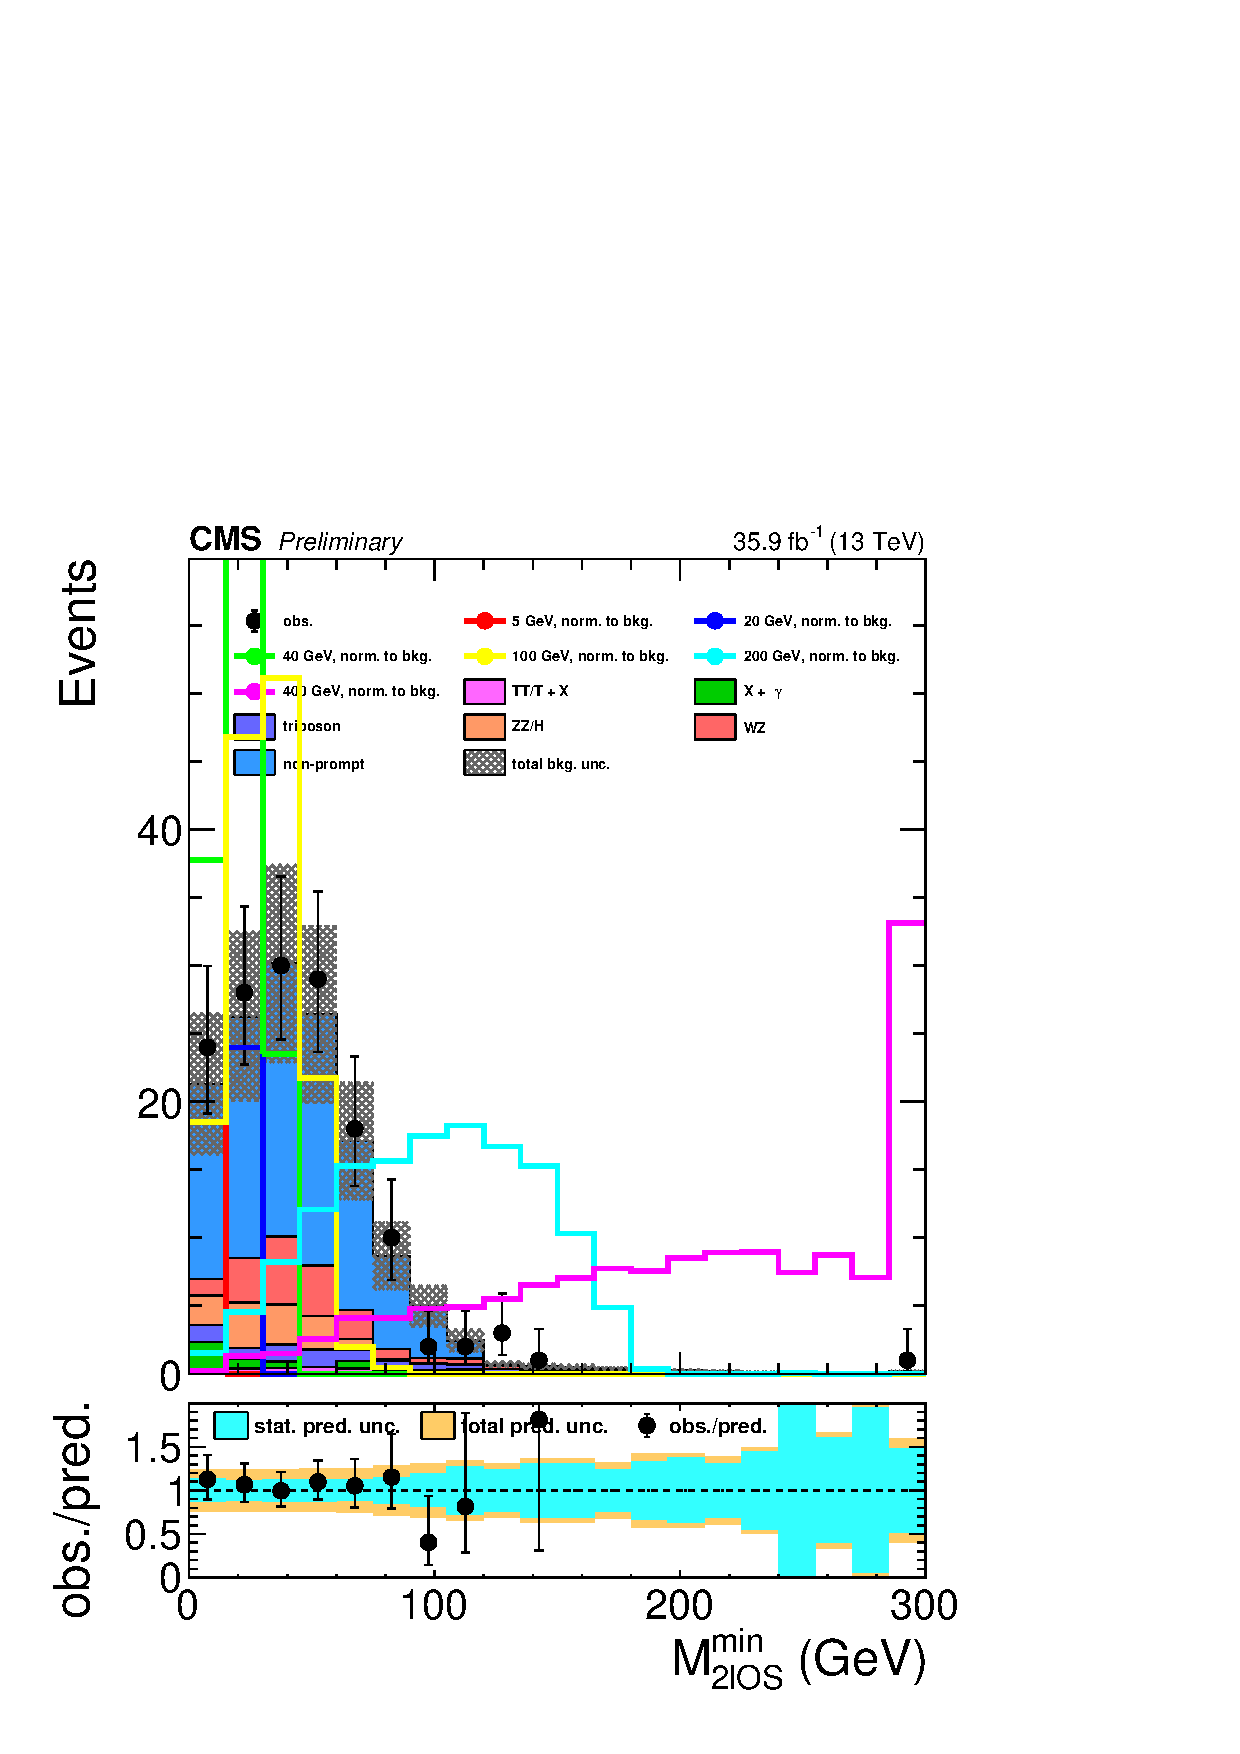
\includegraphics[width=.35\textwidth]{Figures/c5/distribution/minMos_baseline_noOSSF_withSignal.pdf}
  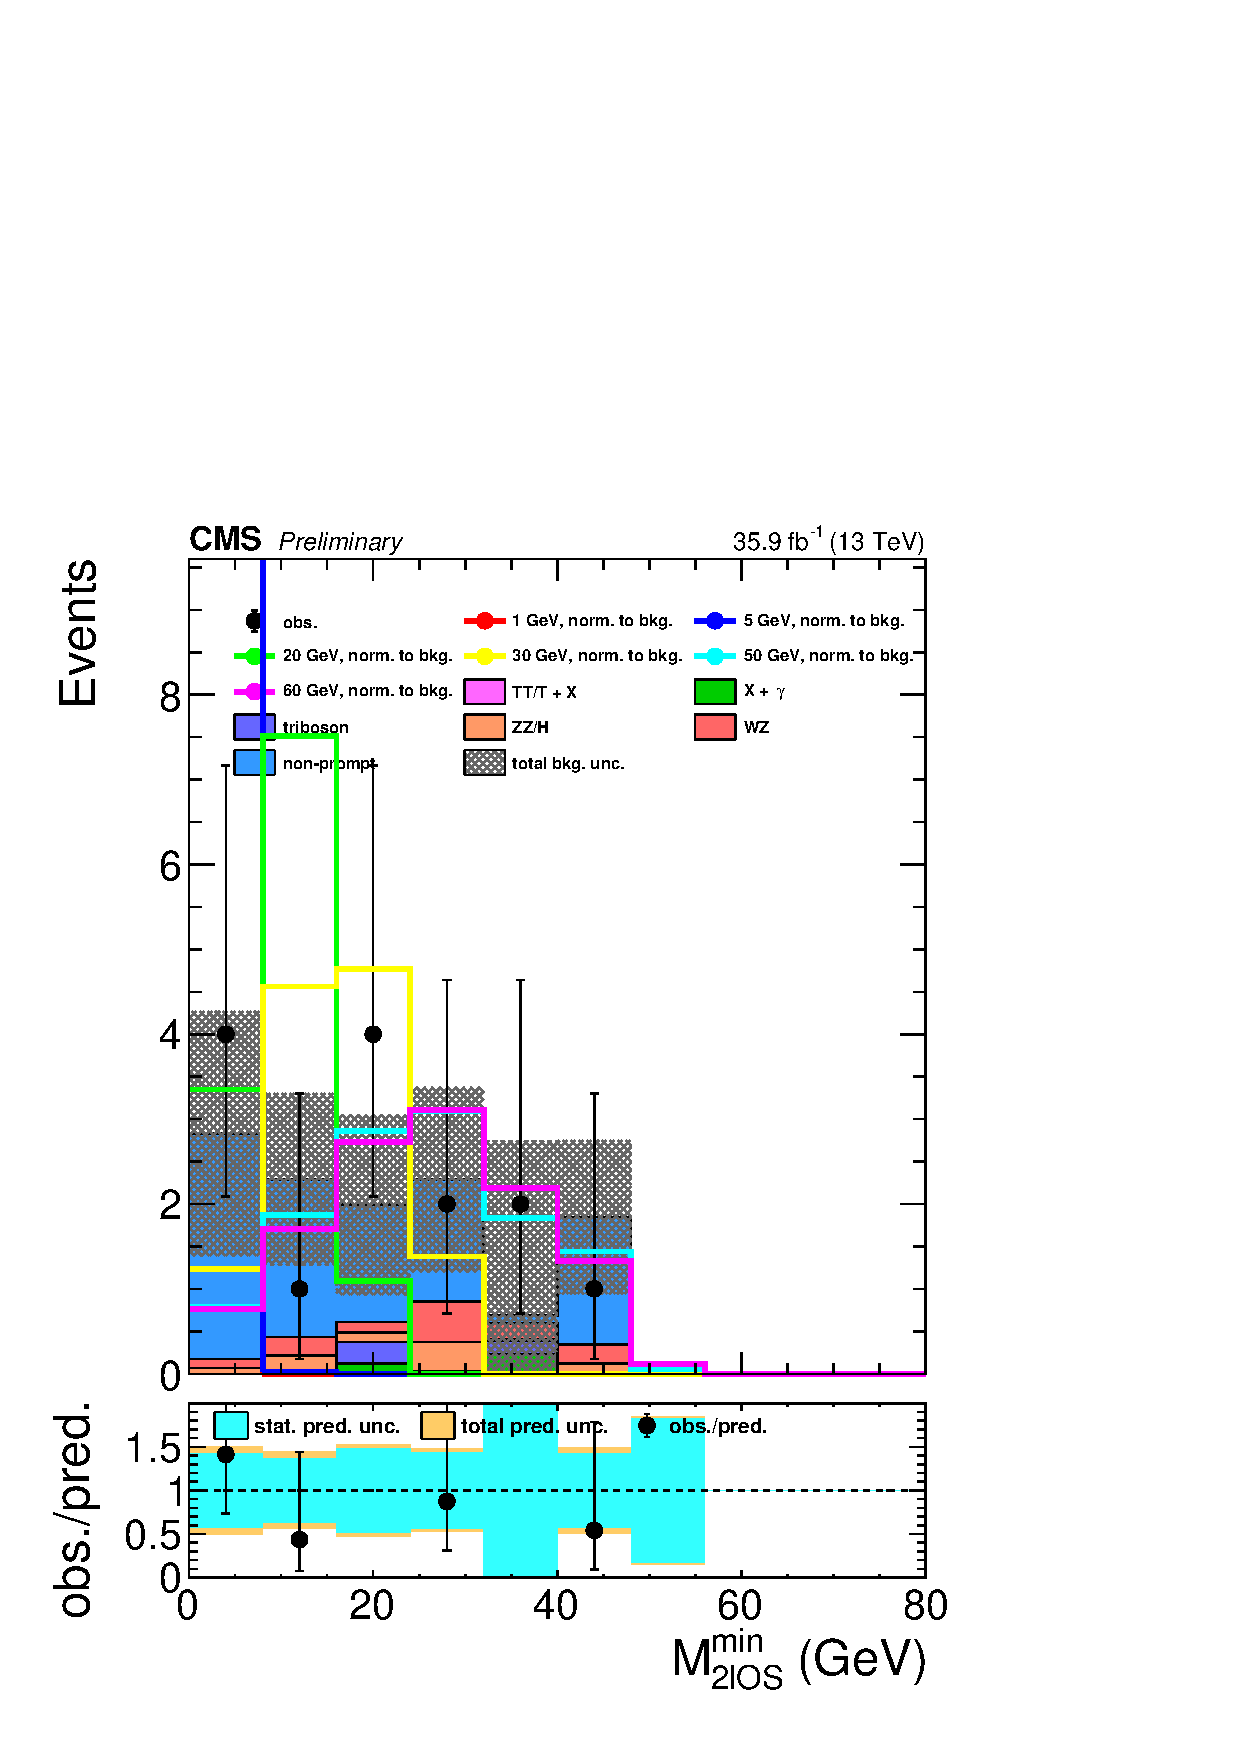
\includegraphics[width=.35\textwidth]{Figures/c5/distribution/minMos_lowM_3lnoOSSF_highPt_withSignal.pdf}
  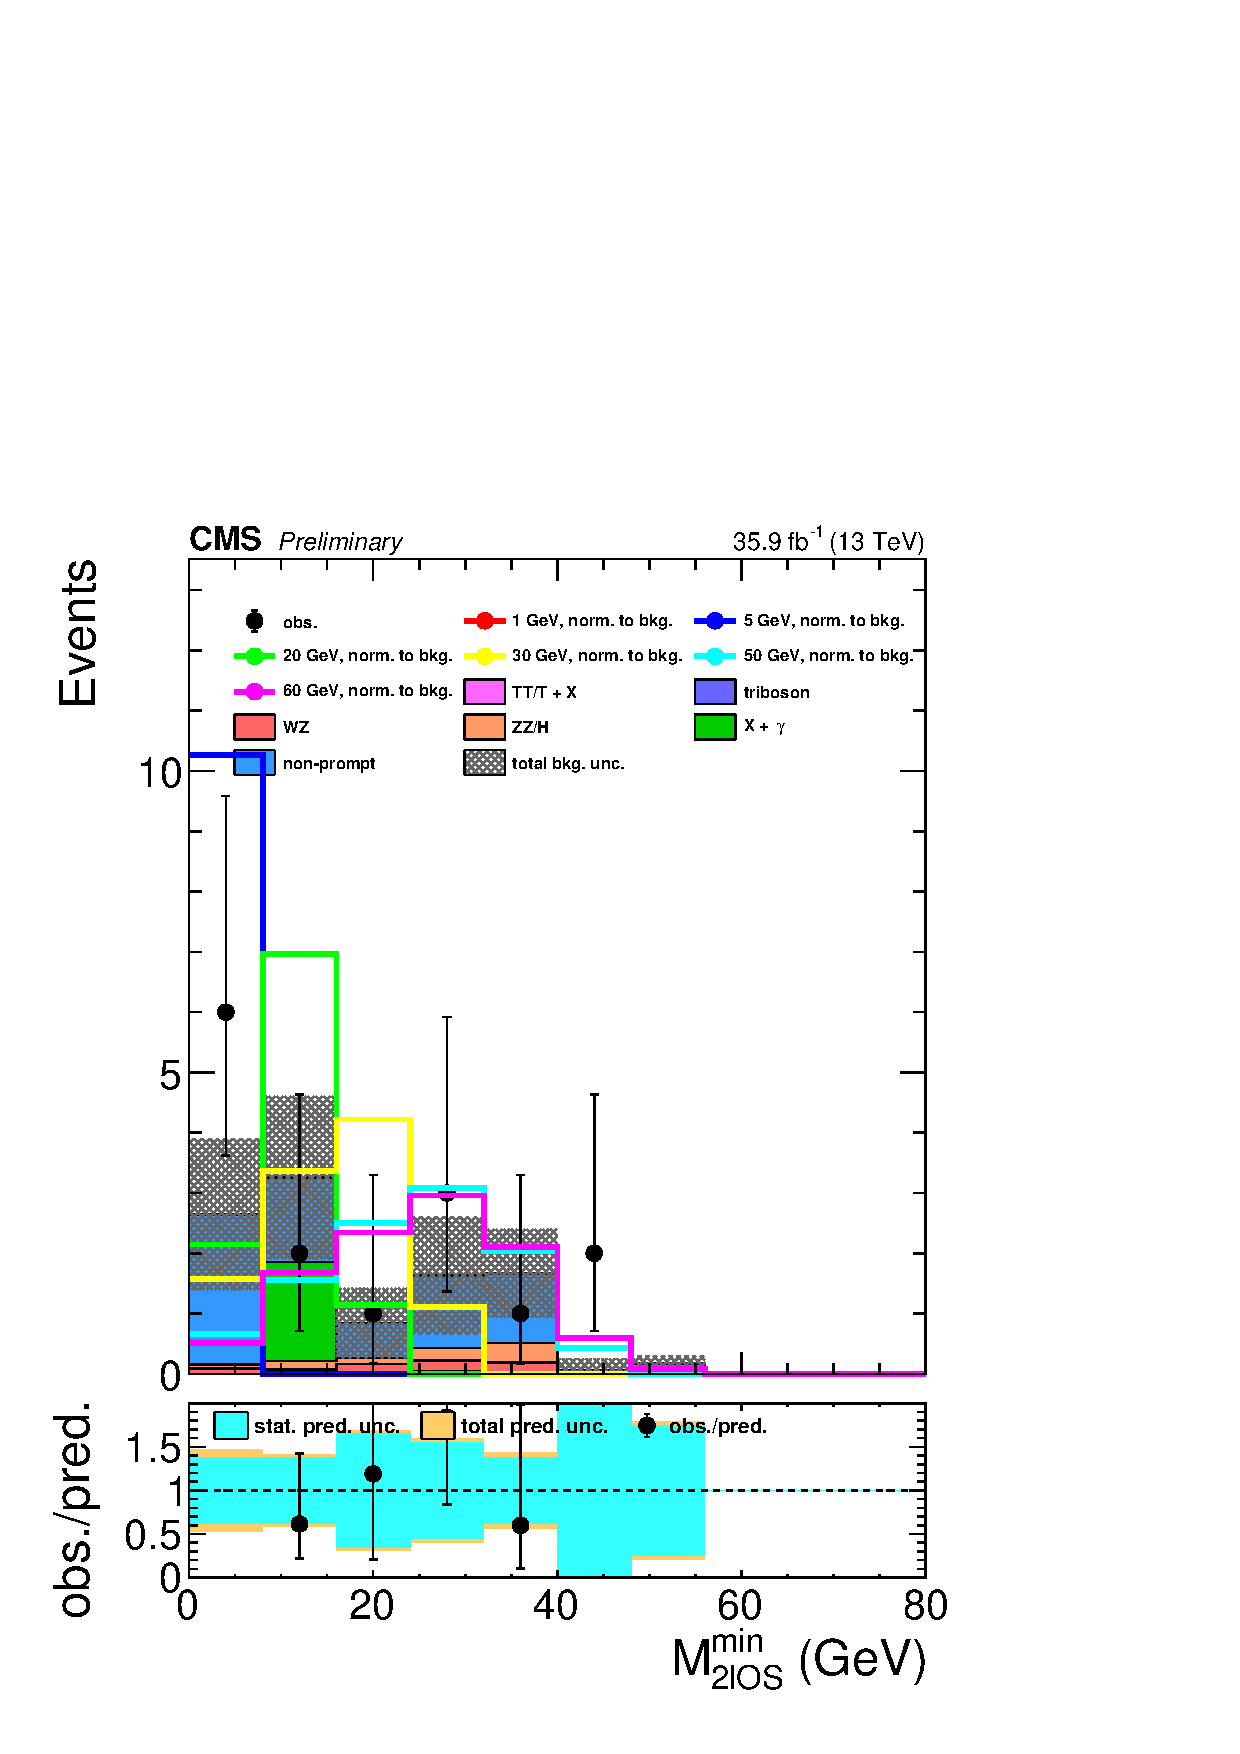
\includegraphics[width=.35\textwidth]{Figures/c5/distribution/minMos_lowM_3lnoOSSF_lowPt_withSignal.pdf}}
  \caption{Expected background yields and signal yields normalized to
  the total background as a function of \mmin for the high leading \pt
  category of the low mass search (middle) and the low leading \pt category
  (right).}
  \label{fig:MminMos}
\end{figure}



The definitions of the low mass
search regions, using this variable, are shown in
Table~\ref{tab:lowMSRdef}. The expected yields in each of these search
regions, compared to the predicted yields of several HNL mass
scenarios, with \mixpar = $10^{-5}$ can be found in the Results
section.  

\begin{table}[tbh]
\centering
\caption{Search regions in the low mass category.}
\label{tab:lowMSRdef}
\resizebox{0.6\textwidth}{!}{
\begin{tabular}{|c|c|c|c|c|}
\hline
\multirow{2}{*}{$\pt^\text{leading}$ (GeV)}  & \multicolumn{4}{ c| } {\mmin  (GeV)} \\\cline{2-5}
 & $ < 10$ & $10 - 20$ & $20 - 30$ & $> 30$\\
\hline\hline
 $ < 30$ &  SR A1 & SR A2 & SR A3 & SR A4\\ \hline
 $30-55$ &  SR B1 & SR B2 & SR B3 & SR B4\\ \hline
\end{tabular}}
\end{table}



\subsection{High mass search}
To facilitate the simultaneous interpretation of the low- and high mass searches, the selection of events entering each search category should be orthogonal. In the low mass search, the following upper limits are applied to several kinematic quantities: 
\ptmiss < 75\GeV, \pt of leading lepton < 55\GeV and \mlll<
80\GeV. Applying a threshold in \met to guarantee orthogonality will
cut away a significant portion of the signal, so we opted for using
either the \pt of the leading lepton or \mlll to require
orthogonality. Both requirements would cut away parts of the signal
for HNL masses that aren't extremely high. By testing both
orthogonality requirements separately, and computing expected
exclusion limits using the search regions defined further,
 it was established that requiring the \pt of the leading lepton to be
 larger than 55 \GeV gave the best performance.
 
In addition to this, the subleading lepton is
 required to pass a \pt threshold of 15\GeV, and the trailing lepton
 is required to be above 10\GeV in \pt .
 This cuts somewhat lower the signal acceptance, but drastically
 reduce the background from fake leptons which is especially large for
 very low trailing lepton \pt values. Events in which an OSSF pair is
 present are rejected if \Mll, defined as the OSSF pair mass closest
 to the \PZ mass, falls within a range of 15\GeV around the \PZ boson
 mass, in order to reject the bulk of the $WZ$ background.
 The same off-\PZ requirement is applied to \mlll in order to suppress
 the contribution from the earlier mentioned asymmetric external and
 internal conversions.

The summary of the \emph{high mass} search event selection is listed
in Table~\ref{tab:highMEventSelectio}.

\begin{table}[h]
  \centering
  \caption{\label{tab:highMEventSelectio} Baseline selection requirements
    applied to all data sets for the \emph{high mass} search. The \pt
    cuts driven by the trigger thresholds are not listed here.}
  \begin{tabular}{l|l}
    \hline
    Variable     & Requirement       \\
    \hline
    \hline
     N. \PQb jets & = 0              \\
    4th $\ell$ vetoe & applied      \\
    $\pt^{leading}$ & > 55 \GeV\\
    $\pt^{subleading}$ & > 15 \GeV\\
    $\pt^{trailing}$ & > 10 \GeV\\
     $|\mlll - 91|$ & > 15\GeV\\
     $|\Mll - 91|$ & > 15\GeV\\
    \mmin & > 5\GeV\\
    \hline
    \hline
  \end{tabular}
\end{table}


In order to minimize the expected exclusion limits on the HNL mixing
parameter we started by checking a plethora of variables for
discriminating power between the signal and the background. The shapes
of the background and that of the signal were compared in all of these
variables, and the most promising variables, giving large and obvious
shape differences were picked out by eye. All the variables displaying
shape differences were then used to design multiple sets of
preliminary search region definitions used for binning the events. The
expected signal exclusion limits were computed for each set of search
regions by performing a simultaneous fit, and compared among the
several preliminary search region definitions. Two variables stood
head and shoulders above the rest, the earlier mentioned \mmin and the
transverse mass of the lepton not belonging to the pair forming this
minimum mass, referred to as \mtmin . In addition \mlll was also seen
to discriminate well between signal and background for very high HNL
masses, but was outperformed by the latter two variables. The expected
yields for all three distributions are plotted in fig.~\ref{fig:mtminmm3lOSSF} for events
with- and without an OSSF pair, compared to several HNL
mass scenarios with yields normalized to those of the background. Note
that in reality the signal to background ratio is larger in the events
without OSSF pairs.

\begin{figure}[h]
\noindent
\makebox[\textwidth]{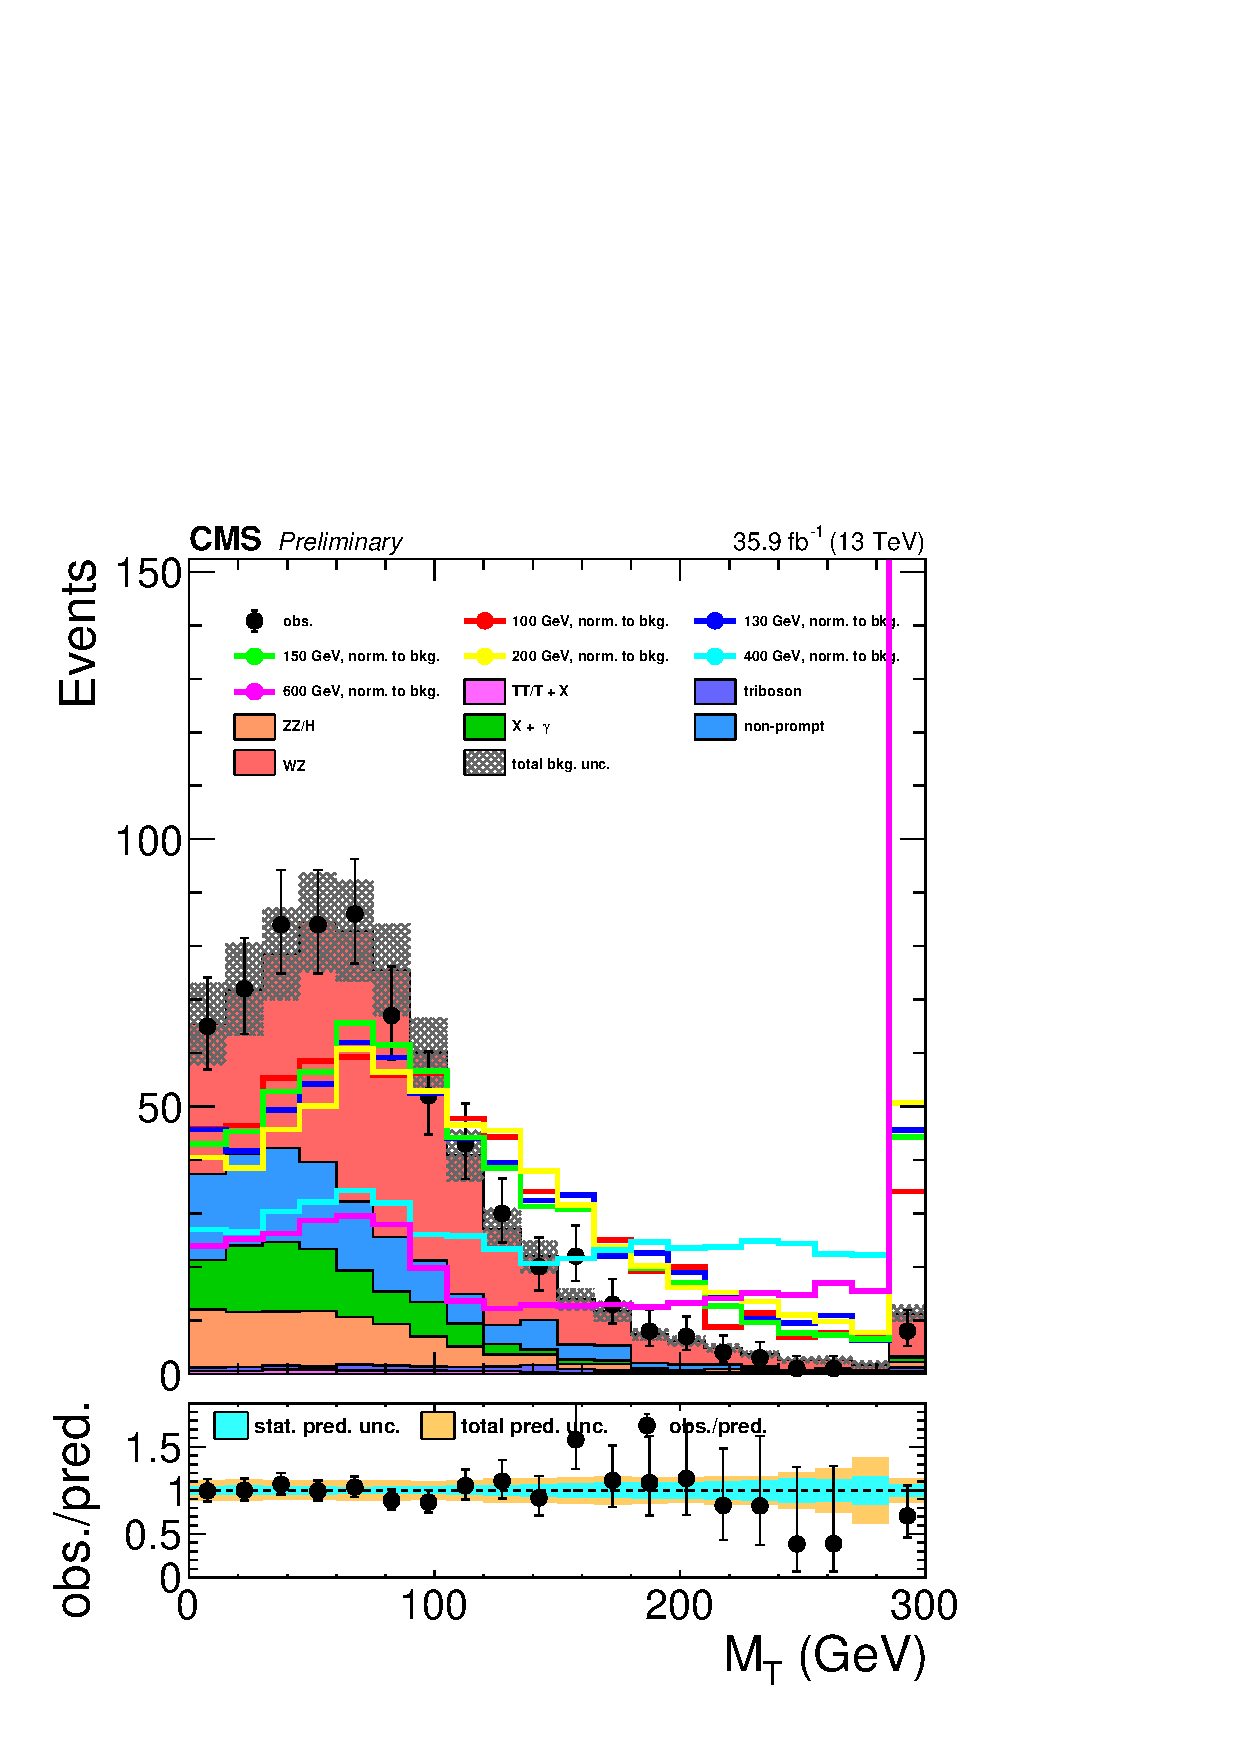
\includegraphics[width=0.3\textwidth]{Figures/c5/distribution/mt_minMos_highM_3lOSSF_withSignal.pdf}
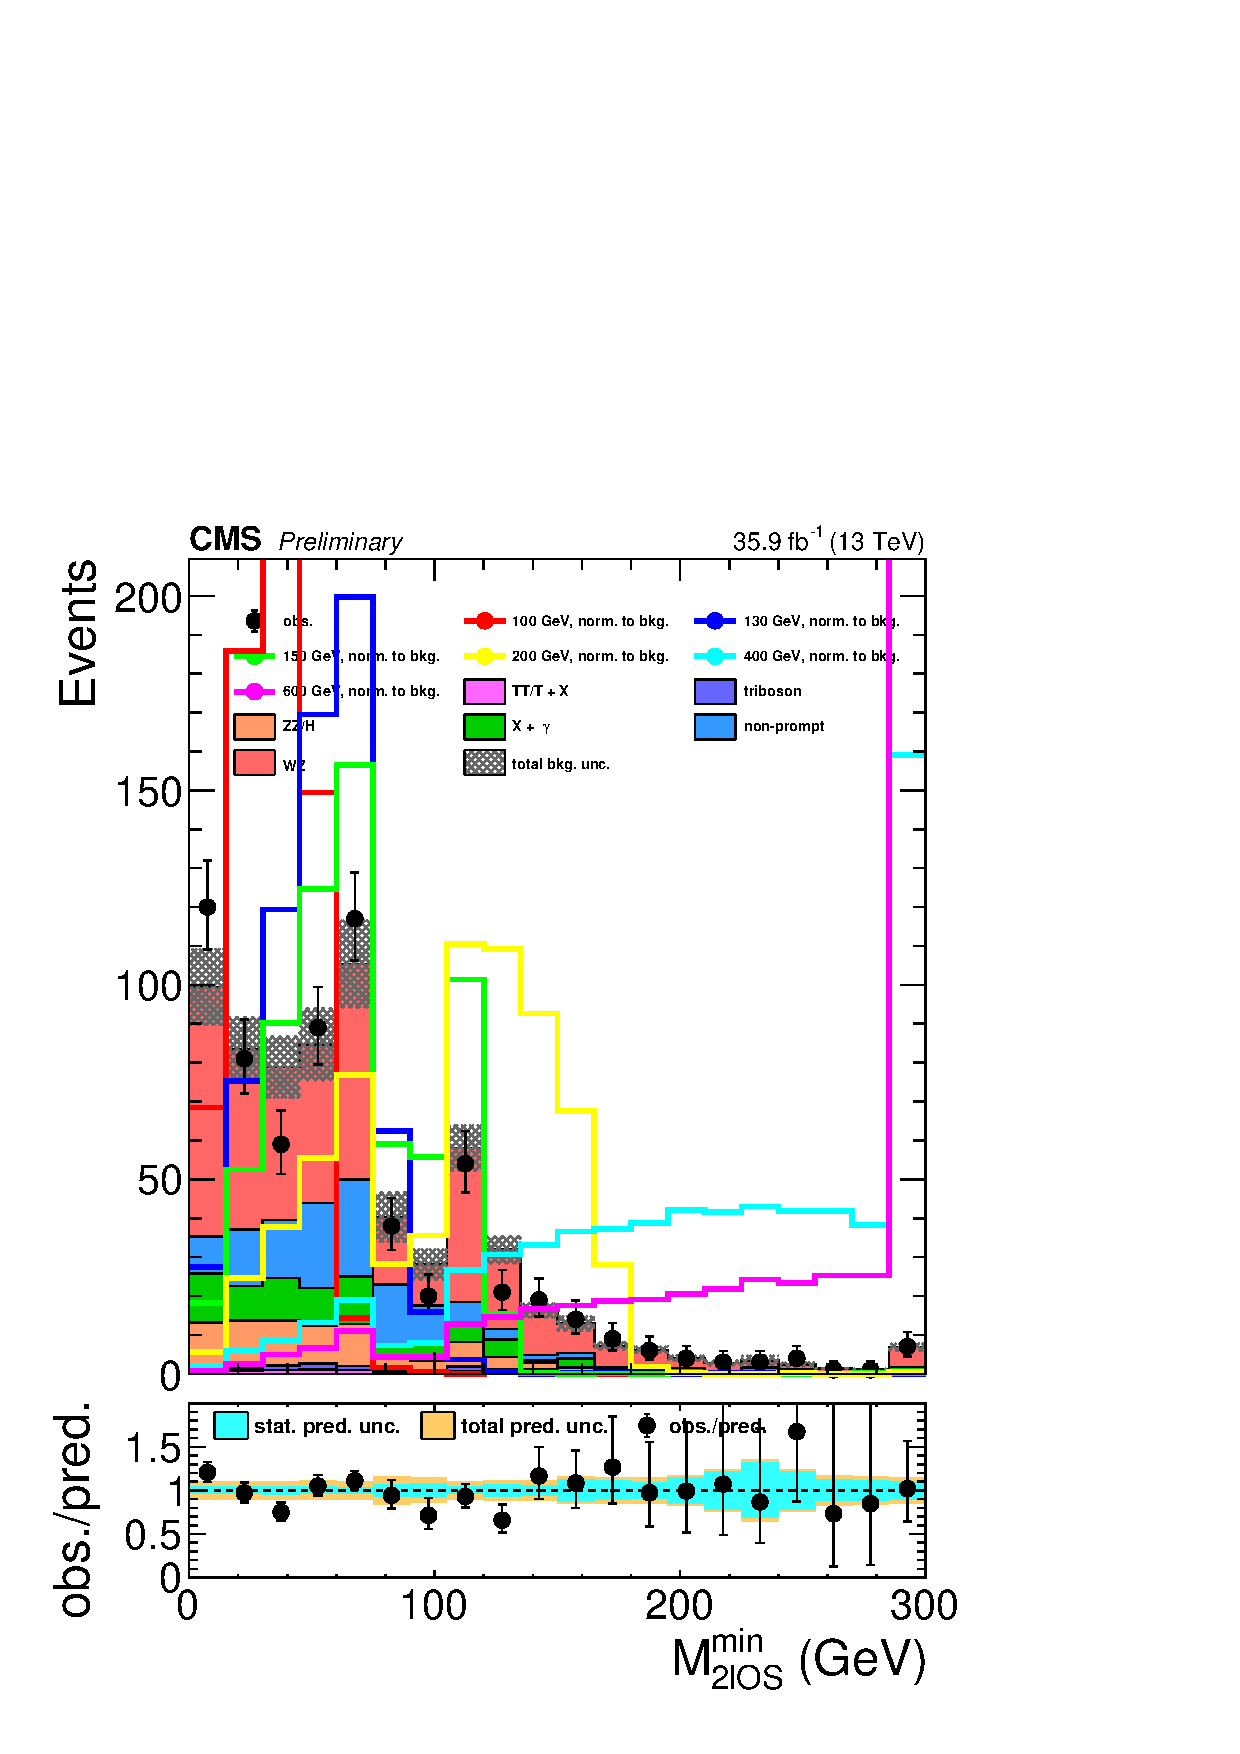
\includegraphics[width=.3\textwidth]{Figures/c5/distribution/minMos_highM_3lOSSF_withSignal.pdf}
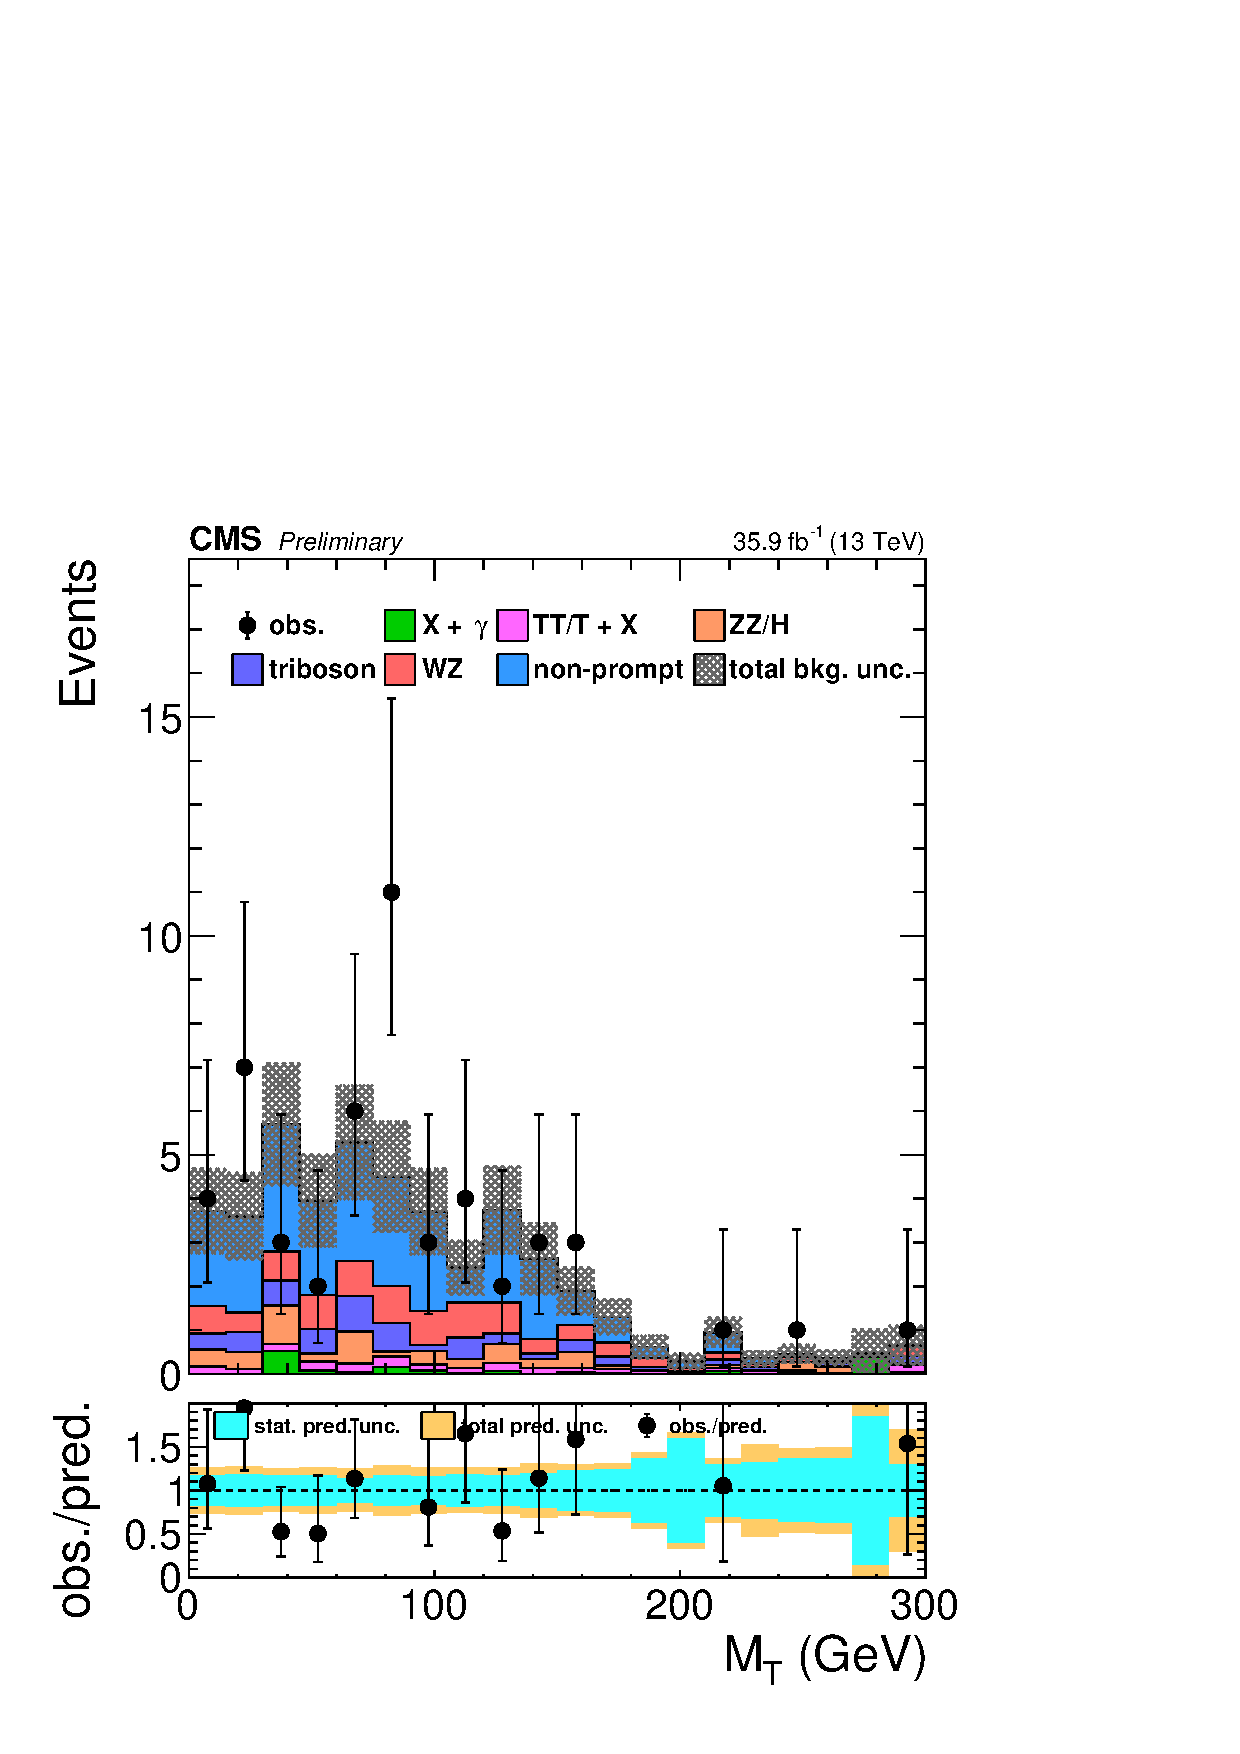
\includegraphics[width=.3\textwidth]{Figures/c5/distribution/mt_minMos_highM_3lnoOSSF.pdf}
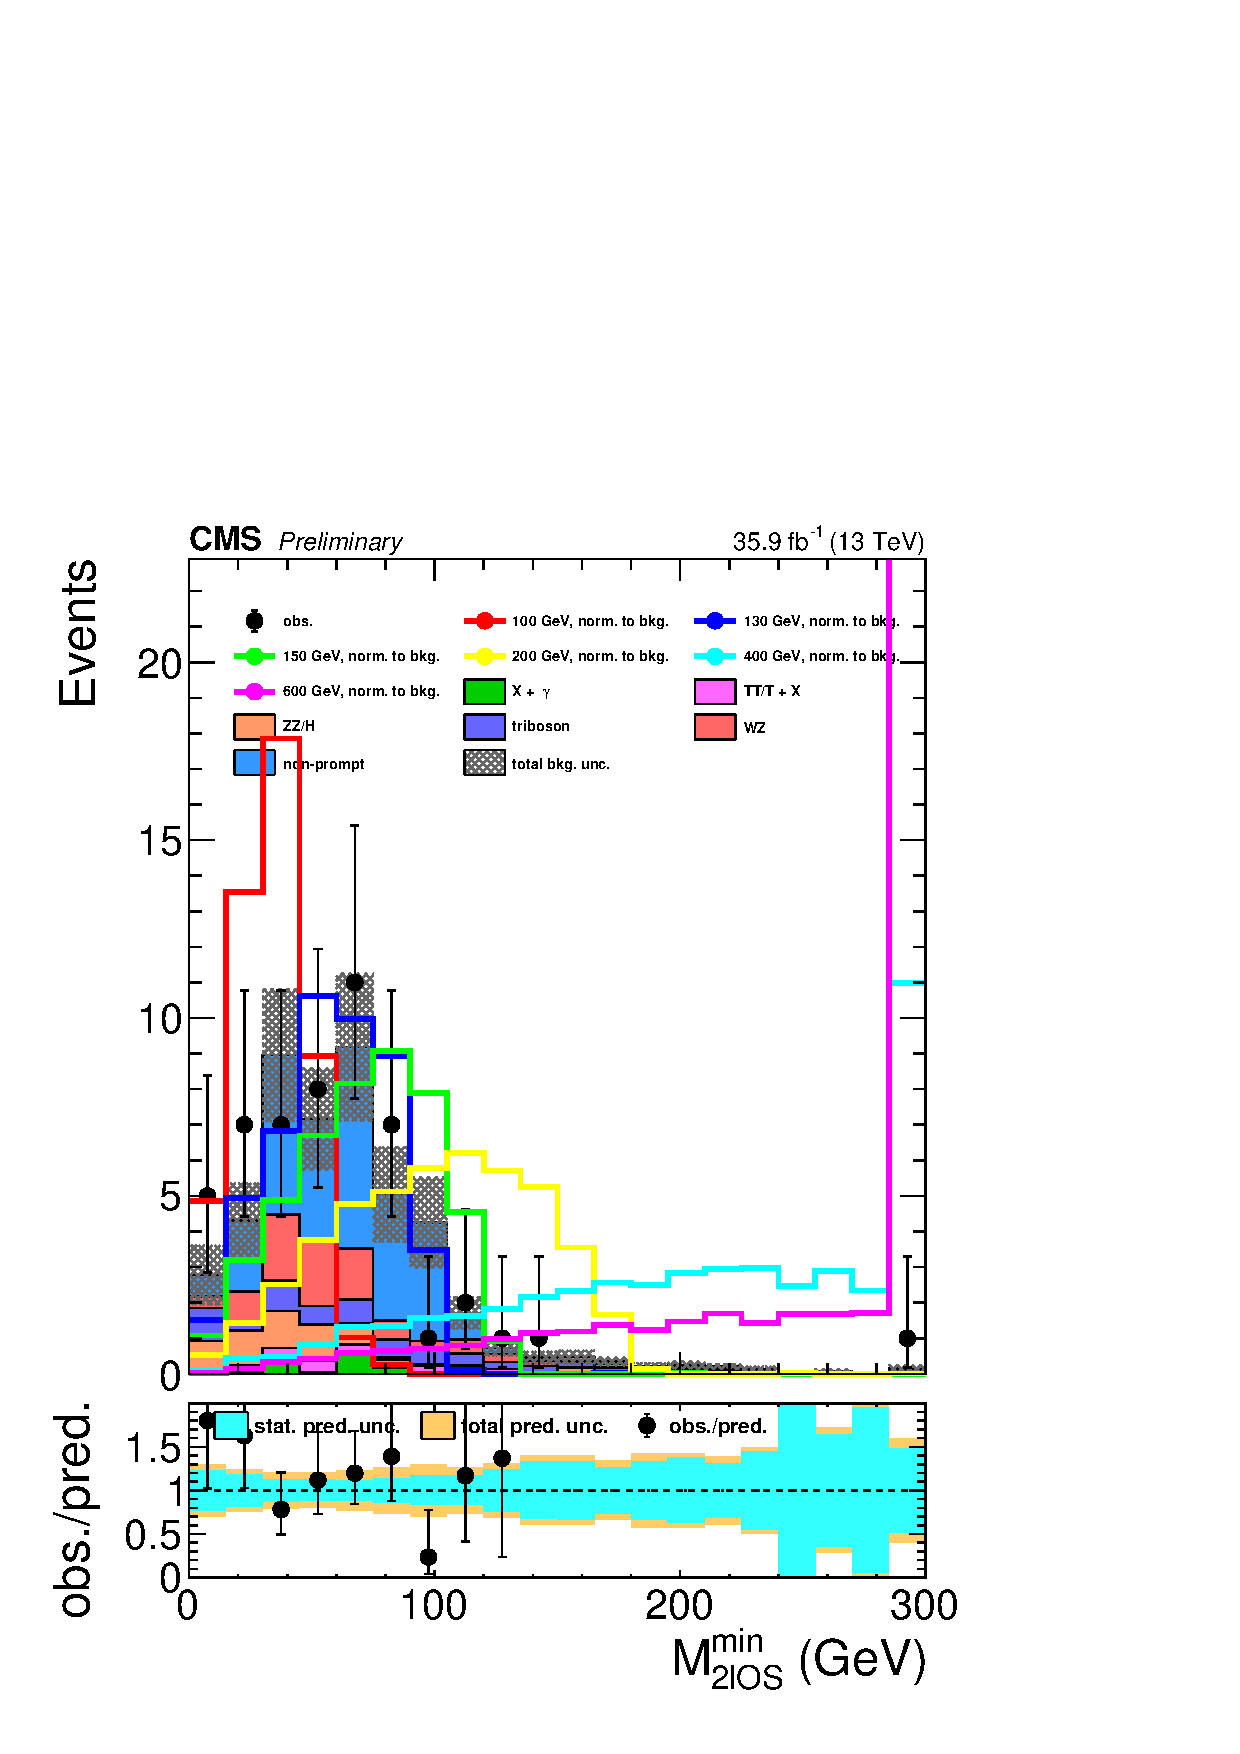
\includegraphics[width=.3\textwidth]{Figures/c5/distribution/minMos_highM_3lnoOSSF_withSignal.pdf}}
\caption{From left to right: The distributions of \mtmin and \mmin for
  events with an OSSF pair (2 left) and without an OSSF pair (2 right)} 
\label{fig:mtminmm3lOSSF}
\end{figure}



Other examples of variables that might be anticipated to be
discriminating between signal and background are \met and the
invariant mass of the 3 lepton + neutrino system, where the
longitudinal momentum of the neutrino is reconstructed from the full
event kinematics. Multiple solutions are possible here, and the
solution for which the reconstructed neutrino mass formed a mass
closest to the W mass with one of the leptons was taken. While \met is
an obvious choice, it wasn't very useful for the signal under
investigation since no extra escaping particles are produced. The 3
lepton + neutrino mass on the other hand gave some discriminating
power, but was found to be far less effective than \mtmin and \mmin.

After it was found that binning search regions in terms of \mtmin and \mmin gave the best performance by leaps and bounds, more refined search regions were defined using these variables. This was done by defining a very large number of search regions, which were iteratively collapsed in order to retain about one background event in each search region, facilitating correct limit setting and a reliable background prediction. Since the total expected event yields in the categories with- and without the presence of an OSSF pair are very different, less separate search regions are defined in the latter than in the former category. In both cases events in with \mlll < 100 \GeV are split off from the rest and binned in terms of \mtmin . This low \mlll bin is expected to give significant contributions to the exclusion of HNL masses below the W mass, and removes a large fraction of the background for high HNL masses. For events with an OSSF pair, events with a pair of loose leptons forming a mass below 5 \GeV are vetoed in order to purify the low \mlll bin from a very large conversion and W$\gamma^{*}$ background. The search region definitions are shown in tables ~\ref{tab:SRhighmassOSSF} and ~\ref{tab:SRhighmassnoOSSF}. The expected background yields as a function of the search region, together with signal yields for several HNL masses at \mixpar = 10$^{-2}$ can be found in the Results section of this text.


\begin{table}[h]
\centering
\caption{Search regions for events with an OSSF pair in the high mass category.}
\label{tab:SRhighmassOSSF}
\resizebox{0.6\textwidth}{!}{
\begin{tabular}{|c|c|c|c|c|}
\hline
\multirow{2}{*}{$\mlll$ (GeV)} & \multirow{2}{*}{\mtmin (GeV)} & \multicolumn{3}{ c| } {$\mmin$  (GeV)} \\\cline{3-5}
 & & $ < 100 $ & $100 - 200 $ & $ > 200$\\
\hline\hline
\multirow{3}{*}{$ 0 - 100$}   & $ < 100$ & \multicolumn{3}{c|}{SR C1} \\ \cline{2-5}
	                         & $100-200$ & \multicolumn{3}{c|}{SR C2} \\ \cline{2-5}
                            & $> 200$ & \multicolumn{3}{c|}{SR C3} \\ \hline
\multirow{6}{*}{$> 100$} & $ < 100  $ & SR C4 & SR C9 & SR C13 \\ \cline{2-5}
				                      & $100-200 $ & SR C5 & SR C10 & SR C14 \\ \cline{2-5}
				                     & $200-300 $ & SR C6 & SR C11 & SR C15 \\ \cline{2-5}
				                      & $300-400 $ & SR C7 & \multirow{3}{*}{SR C12} & \multirow{3}{*}{SR C16} \\ \cline{2-3} 									
									 & $>400$ & SR C8 &  & \\ \hline
\end{tabular}}
\end{table}

\begin{table}[h]
\centering
\caption{Search regions for events without an OSSF pair in the high mass category.}
\label{tab:SRhighmassnoOSSF}
\resizebox{0.6\textwidth}{!}{
\begin{tabular}{|c|c|c|c|c|}
\hline
\multirow{2}{*}{$\mlll$ (GeV)} & \multirow{2}{*}{$\mtmin$ (GeV)} & \multicolumn{3}{ c| } {$\mmin$  (GeV)} \\\cline{3-5}
 & & $ < 100 $ & $100 - 200 $ & $ > 200$\\
 \hline\hline
\multirow{2}{*}{$ 0 - 100$}  & $ < 100$ & \multicolumn{3}{c|}{SR D1} \\ \cline{2-5}
	                         & $> 100$ & \multicolumn{3}{c|}{SR D2} \\ \hline     
\multirow{4}{*}{$> 100$} & $ < 100  $ & SR D3 & SR D7 & \multirow{4}{*}{SR D9} \\ \cline{2-4}
				                      & $100-150 $ & SR D4 & \multirow{3}{*}{SR D8} &  \\ \cline{2-3}
				                      & $150-250 $ & SR D5 & & \\ \cline{2-3}
				                      & $> 250$ & SR D6  & & \\ \hline								
\end{tabular}}
\end{table}

	
\clearpage




\section{Background estimation}
\subsection{}
\subsection{}
\subsection{}
\subsection{}
\subsection{}

\section{Systematic uncertainties}
\section{Results}
\subsection{Low mass results}
\subsection{High mass results}
\subsection{Summary}

\section{Interpretation}
\subsection{Lifetime correction to upper limits}

\section{Conclusion}
